% Canonical NeurIPS 2026 Evaluations & Datasets submission.
% Build from the repository root with `make neurips`.
\documentclass{article}
\usepackage[eandd,nonatbib]{neurips_2026} % double-blind review version

\usepackage{graphicx}
\usepackage{booktabs}
\usepackage{amsmath}
\usepackage{amssymb}
\usepackage{hyperref}
\usepackage{caption}
\usepackage{subcaption}
\usepackage{xcolor}
\usepackage{float}
\usepackage{placeins}
\usepackage{multirow}
\usepackage{amsthm}
\usepackage{enumitem}
\usepackage{algorithm}
\usepackage{algpseudocode}

\newtheorem{corollary}{Corollary}
\newtheorem{lemma}{Lemma}
\newtheorem{observation}{Observation}
\theoremstyle{remark}
\newtheorem{remark}{Remark}

\title{Diagnosing Temporal Sensitivity in Video Retrieval Pipelines}

% Replace with the final author block only after double-blind review.
\author{Anonymous Author(s)}

\begin{document}
\maketitle

\begin{abstract}
Scalable video retrieval often uses global descriptors that are insensitive to motion
direction. Two videos of the same road in opposite directions, or left versus right turns
at the same intersection, can therefore receive similar scores without exposing the
failure in an aggregate retrieval metric. We introduce three executable diagnostics: a
temporal scramble gradient ($K\!\in\!\{1,\ldots,16\}$), a forward/reverse test with a
comparator-specific reversal score $s_\text{rev}$, and a controlled feature--comparator
factorial. Across seven benchmarks and three open-weight VLMs, the diagnostics distinguish
exact permutation invariance of independently encoded frame sets from empirical
near-invariance of contextual representations. On Honda HDD, replacing pooled cosine by
per-frame dynamic time warping closes 89\% of the observed pair-classification AP gap between a
V-JEPA~2 bag-of-tokens baseline and its temporal residual, with a paired cluster-bootstrap
difference of $+0.117$ [0.044, 0.127]. However, the ranking reverses in corrected global
retrieval (DTW 0.177 vs. bag-of-tokens 0.256 mAP). nuScenes supports the conditional pair
contrast, while Something-Something V2 favors a different representation and comparator.
VLM results are readout- and prompt-dependent: sequence comparisons expose
forward/reverse changes that pooling suppresses, direct direction prompts are weak, and
an integrity prompt can classify the same clips well. We consolidate the observed failure
modes into a taxonomy and executable protocol, and release a toolkit implementing all
three diagnostics. The results identify a task-dependent tension between scalable
invariant matching and temporal discrimination, rather than an intrinsic blindness of
all video architectures.
\end{abstract}

\section{Introduction}

Global video descriptors can collapse motion direction: cars driving the same road in opposite directions may retrieve as near-duplicates, and left and right turns at the same intersection can receive similar scores. A common scalable first stage is the \emph{bag-of-frames} (BoF) construction, which mean-pools independently encoded frame embeddings~\cite{faiss, semdedup} and therefore discards order exactly. Such invariant matching is useful in Video Copy Detection (VCD; finding re-encoded, cropped, or camcorded copies), while motion-aware applications require a different comparison. Modern VCD systems also use frame-level localization and sequence matching, so our claim concerns this specific global-descriptor construction rather than the field as a whole.

Temporal blindness is well documented for generative \emph{question answering} (QA)~\cite{tomato,temporalbench,tempcompass,infact,videozerobench,vbenchcomp}: probes score near chance on temporal tasks, and frame shuffling leaves benchmark scores intact. These diagnoses surface in text. In retrieval, they surface in nothing: the vector database returns the same neighbor, and the user never sees the failure. We study three regimes where the value of temporal order flips:

\textbf{1. Scene matching (order irrelevant):} for VCD and scene retrieval (e.g., ``activities in different rooms''), the discriminative cue is visual appearance. Semantic pooling suffices; temporal invariance is a feature.

\textbf{2. High-overlap motion retrieval (order is the signal):} querying a dashcam fleet for ``left turns at Intersection X'' requires encoding motion dynamics. Left and right turns share the same intersection (the static background), so BoF collapses them to the same point.

\textbf{3. Temporal manipulation (order as diagnostic):} reversing a video yields BoF similarity $1.0$ to its source. This is both a clean stress test for whether a representation has any temporal sensitivity and, secondarily, a copy-detection vulnerability~\cite{fojcik2025}.

Beyond retrieval, temporal order is a prerequisite for any predictive representation~\cite{lecun_worldmodel}. A model that cannot distinguish forward from reverse cannot forecast future states. We return to this connection as an implication in Section~\ref{sec:discussion}, but our scope here is diagnostic, not architectural.

We evaluate these cases with two primary encoders, DINOv3~\cite{dinov3} (image-SSL ViT-L; BoF and DTW attention trajectories) and V-JEPA~2~\cite{vjepa2} (spatiotemporal prediction residuals). Three temporal-training controls probe whether specialized objectives help: ViCLIP~\cite{viclip} (video-native contrastive), TARA~\cite{tara} (a multimodal LLM fine-tuned with chirality, i.e. mirror direction, negatives), and PL-Stitch~\cite{plstitch} (Plackett-Luce temporal ranking). Three VLMs (Qwen3-VL~\cite{qwen3vl}, Gemma~4~\cite{gemma4}, LLaVA-Video~\cite{llavavideo}) probe whether LLM backbones preserve temporal signal. Benchmarks span seven domains, including VCDB~\cite{vcdb} (near-duplicate video copy detection), Honda HDD~\cite{honda_hdd} (ego-vehicle driving maneuvers), nuScenes~\cite{nuscenes} (autonomous driving), Something-Something V2~\cite{ssv2} (crowd-sourced tabletop manipulation; non-driving cross-domain test), Nymeria~\cite{nymeria} (egocentric daily activity), MUVR~\cite{muvr} (multi-modal untrimmed video retrieval), and EPIC-Kitchens-100~\cite{epickitchens} (egocentric kitchen procedures).

\textbf{Contributions.} This paper introduces a diagnostic framework for temporal sensitivity in video retrieval, comprising three executable instruments: (1)~a \emph{temporal scramble gradient} separating methods with detected order sensitivity from methods that remain flat (Figure~\ref{fig:scramble_gradient}); (2)~a \emph{forward--reverse test} producing a comparator-specific reversal score $s_\text{rev}$; and (3)~a \emph{feature--comparator factorial} that evaluates both factors on one shared pair set. Applied across seven benchmarks and three open-weight VLMs, the framework localizes where temporal information is preserved or suppressed, and consolidates findings into a 10-mode taxonomy and executable classification protocol (Appendix~\ref{sec:failure_taxonomy}, Algorithm~\ref{alg:decision}).

\section{Methods}
\label{sec:methods}

\textbf{Why BoF is blind.}
Mean-pooling a fixed set of representations is permutation-invariant: $g(f_1, \ldots, f_T) = g(f_{\pi(1)}, \ldots, f_{\pi(T)})$ for any permutation $\pi$~\cite{deepsets}. Thus BoF over independently encoded frames is exactly invariant, as are max pooling and Chamfer matching on the same fixed frame set. The theorem does \emph{not} imply that pooling contextual tokens from a video encoder is invariant to reordering the raw frames, because the token values can themselves change with order. For those representations, invariance is an empirical result rather than an architectural guarantee.

\textbf{Feature-vs-comparator decomposition.}
We distinguish the encoder (\emph{features}) from the \emph{comparator}, the full similarity function (cosine over BoF, DTW over per-frame sequences, etc.). The aggregator is one stage inside the comparator. We evaluate the feature $\times$ comparator factorial on one shared pair set, fixing one factor while varying the other. This controlled comparison localizes performance differences but does not, by itself, establish a causal attribution.

\textbf{DINOv3 \& Attention Trajectories.} We extract 1024-d CLS embeddings per frame from DINOv3 ViT-L~\cite{dinov3}. \emph{BoF} mean-pools frame embeddings into a single vector, compared via cosine similarity. \emph{Chamfer similarity}~\cite{kordopatis2019visil} computes the pairwise frame similarity matrix and averages the symmetric maximum: $\frac{1}{2}\bigl(\mathrm{mean}_i \max_j S_{ij} + \mathrm{mean}_j \max_i S_{ij}\bigr)$, remaining order-invariant while retaining per-frame structure. For structural tracking, we compute the spatial center-of-mass of the CLS$\to$patch attention map (last layer, averaged across heads) per frame, yielding a 2D trajectory compared via DTW. Temporal derivatives of CLS embeddings capture changes between adjacent frames and are also compared via DTW.

\textbf{V-JEPA~2 Temporal Residuals.} V-JEPA~2 ViT-L~\cite{vjepa2} ingests 64 frames as $32 \times 16 \times 16$ spatiotemporal patches ($D\!=\!1024$). The \emph{prediction residual} $R = \hat{P} - P$ (predicted minus actual masked patches) captures prediction-error patterns. We spatially average each temporal position to obtain $\bar{R} \in \mathbb{R}^{T_\text{mask} \times D}$, independently min--max normalize each feature dimension over time within each sequence, and compare sequences via DTW with similarity $\exp(-d_\text{DTW})$. The \emph{bag-of-tokens} (BoT) baseline mean-pools all contextual encoder patches into a single vector (cosine similarity); its behavior under reversal is measured rather than inferred from symmetry.

\textbf{Temporal Scramble Gradient.} We split video~B's frame embeddings into $K$ near-equal chunks (sizes differ by at most one), randomly shuffle them, and reassemble. Sweeping $K \in \{1, \ldots, 16\}$ traces a gradient from intact to more finely scrambled. We shuffle \emph{extracted} embeddings (see Appendix~\ref{sec:scramble_data}). A decreasing curve is evidence of sensitivity in the comparator; a flat curve means that this intervention detected no sensitivity, not that invariance has been proved.

\textbf{VLM Generative Probes.} We present forward and reversed clips to VLMs under three semantically equivalent prompts and report mean balanced accuracy $(\mathrm{TPR}+\mathrm{TNR})/2$ averaged over prompts. Reported $\pm$ is prompt-sensitivity standard deviation, not statistical uncertainty (binomial 95\% CI at $N\!=\!200$ is $\pm 0.035$).

\textbf{ViCLIP.} ViCLIP ViT-L~\cite{viclip}, trained contrastively on 10M video clips, jointly encodes 8 frames via temporal attention into a single 768-d embedding (cosine similarity).

\textbf{TARA.} TARA~\cite{tara} fine-tunes a Tarsier-7B multimodal LLM with chiral (mirror-direction) negatives for temporal retrieval, encoding 16 frames into a single 4096-d vector via end-of-line prompting (cosine similarity).

\textbf{PL-Stitch.} PL-Stitch~\cite{plstitch} pretrains a ViT-Base (86M params) with Plackett-Luce temporal ranking, producing per-frame 768-d CLS-token embeddings that support the same feature-vs-comparator decomposition as DINOv3: BoF, Chamfer, temporal derivative DTW, and DTW on raw embeddings.

\textbf{VLM Embedding Probes.} These are \emph{diagnostic procedures}, not new models: each probe reads a representation from an existing VLM pipeline and emits a descriptive $s_\text{rev}$ value. We probe three stages: (1)~\emph{vision pooled}, the mean-pooled vision tower output (frame$\times$patch tokens); (2)~\emph{vision sequence}, per-frame pooled vision tokens as a $(T, D)$ sequence compared via temporal derivative DTW; (3)~\emph{LLM hidden state}, the mean-pooled last-layer hidden state over all input tokens. We ask how similar a clip's representation is to the representation produced for its reversed version. A cosine value of 1.0 indicates identical direction after normalization for that pooled comparator; lower DTW-derived values indicate larger sequence differences on that comparator's own scale. Formally, for representations $\mathbf{z}$ (single vector) or $\mathbf{Z}$ (sequence of vectors):
\begin{equation}
s_\text{rev} =
\begin{cases}
\cos(\mathbf{z}_\text{fwd},\; \mathbf{z}_\text{rev}) & \text{pooled probes (single vector),} \\[4pt]
\exp\!\bigl(-\alpha \cdot d_\text{DTW}(\mathbf{Z}_\text{fwd},\; \mathbf{Z}_\text{rev})\bigr) & \text{sequence probes (temporal derivative DTW),}
\end{cases}
\label{eq:srev}
\end{equation}
where $\alpha$ follows the DTW $\alpha$ schedule defined below. Raw $s_\text{rev}$ values exceeding 1.0 (from f32 cosine precision) are clamped to 1.000 in all tables and figures; affected entries are marked $^\dagger$.
\begin{remark}[Cross-family comparability]
\emph{Pooled} $s_\text{rev}$ (cosine) and \emph{sequence} $s_\text{rev}$ ($\exp(-\alpha d_\text{DTW})$) use different similarity functions and are \textbf{not directly comparable}. Even within the DTW family, preprocessing and $\alpha$ determine the numerical scale. We therefore use $s_\text{rev}$ descriptively within a fixed probe definition and do not construct a cross-method frontier from it.
\end{remark}

\textbf{DTW Implementation.} Dynamic time warping aligns two sequences via a minimum-cost monotonic path that can stretch time but not reverse it, so it penalizes some order violations that pooled cosine ignores. All comparisons use unconstrained warping with L2 cost matrices, accumulated-cost normalization by $T_1 + T_2$, and GPU-vectorized anti-diagonal wavefront processing~\cite{ddtw}. For residuals and encoder sequences, each sequence and feature dimension is independently min--max normalized over time; attention trajectories are likewise normalized to $[0,1]$. Similarity is $\exp(-\alpha \cdot d_\text{DTW})$ with $\alpha = 1$ for derivatives/residuals and $\alpha = 5$ for attention trajectories. Because this transform is monotone for fixed $\alpha$, AP rankings are invariant to $\alpha$ for one distance matrix; the similarity values themselves are not.

\section{Experiments and Results}

\textbf{Evaluation protocols.} We report average precision (AP; area under the precision--recall curve) and, where applicable, area under the ROC curve (AUC). Except for the explicitly identified reranking experiment, these are pooled pair-classification diagnostics, not standard query-wise retrieval metrics. \emph{VCDB}: 528 videos; 5{,}585 positive pairs from annotations, negatives sampled 1:1 with fixed seed (sensitivity analysis across 1:1, 1:5, and all-pairs in Appendix~\ref{sec:neg_sampling}). \emph{HDD}: all $\binom{n}{2}$ pairs within each GPS-clustered intersection (DBSCAN density clustering, $\epsilon\!\approx\!30$\,m); positive = same maneuver; 50 mixed clusters, 1{,}687 maneuvers. \emph{nuScenes}: same protocol on ego\_pose; CAN-bus (Controller Area Network) turn labels; 264 segments, 950 pairs. \emph{EPIC s\textsubscript{rev}}: per-sequence self-comparison on 500 sequences; bootstrap 95\% CIs (1{,}000 resamples). \emph{Nymeria}: 100 egocentric sessions, 8{,}780 segments; positive = same activity same room; all $\binom{n}{2}$ pairs (394{,}210). \emph{MUVR News}: 9{,}958 videos, 74 topics, 27{,}453 positive pairs. \emph{SSv2}: 400 clips across chiral (mirror-direction) template pairs---e.g., ``pushing left to right'' vs.\ ``pushing right to left''---50 per template; within-pair pairwise evaluation where positive = same template and negative = chiral twin.

\subsection{VCDB Reversal Diagnostics}

On copy detection, BoF and Chamfer dominate. DINOv3 Chamfer reaches AP\,=\,0.989 (528 videos, 5{,}585 positive pairs), while temporal methods underperform on frame-to-frame intra-class noise. Individual VCDB AP values swing by ${\pm}0.06$ across random negative seeds (Appendix~\ref{sec:neg_sampling}), but rank order is preserved. Nymeria and MUVR replicate the ranking (Appendix~\ref{sec:scene_matching}).

Order-invariance is also a vulnerability, since reversed video yields identical BoF similarity. We measure this across VCDB positive pairs:

\begin{table}[ht]
\centering
\caption{VCDB Reversal Attack: 5{,}585 positive pairs (AP drop indicates detection of evasion). Bar-chart visualization in Appendix~\ref{sec:reversal_figure}.}
\label{tab:vcdb_reversal_attack}
\begin{tabular}{lccc}
\toprule
\textbf{Method} & \textbf{Normal AP} & \textbf{Reversed AP} & \textbf{AP $\Delta$} \\
\midrule
Chamfer (DINOv3) & 0.989 & 0.989 & \textbf{-0.000} (Invariant) \\
BoF (DINOv3) & 0.979 & 0.979 & \textbf{-0.000} (Invariant) \\
BoT (V-JEPA 2) & 0.838 & 0.832 & -0.006 \\
\textbf{Attention Trajectory (DINOv3)} & 0.700 & 0.542 & \textbf{-0.158} (Detects) \\
Temporal Residual (V-JEPA 2) & 0.698 & 0.631 & -0.067 \\
\bottomrule
\end{tabular}
\end{table}

BoF and Chamfer yield zero AP delta under reversal. Only attention-trajectory DTW flags the reversed copy ($\Delta = -0.158$); the temporal residual registers a smaller drop ($\Delta = -0.067$). To move beyond this binary test, we apply chunk-shuffle scrambling at varying granularity ($K \in \{1, \ldots, 16\}$).

\begin{figure}[ht]
    \centering
    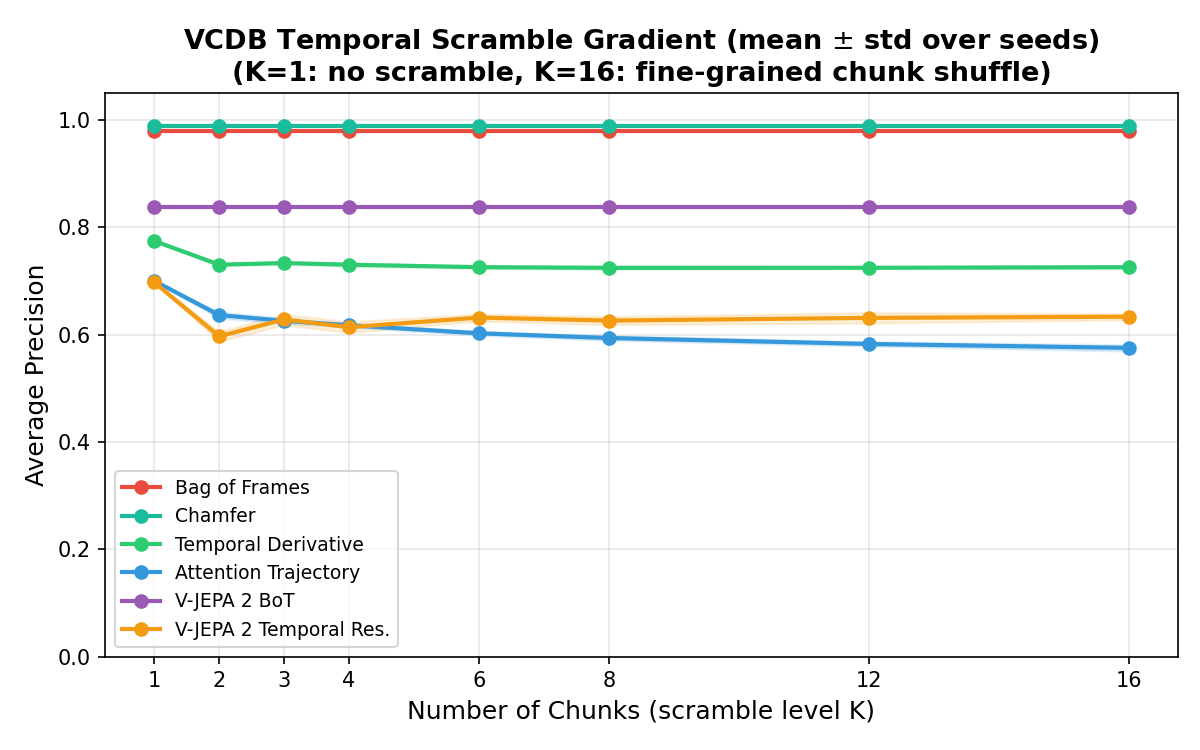
\includegraphics[width=0.9\textwidth]{../figures/vcdb_scramble_gradient_errorbars.png}
    \caption{Corrected temporal scramble gradient on VCDB using near-equal chunks and 10 shuffle seeds per $K$. BoF, Chamfer, and V-JEPA~2 BoT remain flat; sequence comparators decline, with standard deviation at most 0.0101 (Appendix~\ref{sec:scramble_data}).}
    \label{fig:scramble_gradient}
\end{figure}

With the corrected partitions, exact fixed-set comparators remain flat: BoF stays at AP\,=\,0.979 and Chamfer at 0.989, while contextual BoT is empirically flat at 0.837. Attention-trajectory AP falls from 0.700 to 0.575 and temporal-derivative AP from 0.775 to 0.726. The V-JEPA~2 residual drops sharply after the first shuffle and ends at 0.633, but is non-monotonic across intermediate $K$; the diagnostic detects sensitivity without supporting a monotonic-severity claim.

\subsection{High-Overlap Motion: Honda HDD \& nuScenes}
\label{sec:motion}

To isolate motion from appearance, we clustered 128 Honda HDD~\cite{honda_hdd} driving sessions by RTK GPS (Real-Time Kinematic differential positioning, ${\sim}2$\,cm accuracy), extracting 1{,}687 maneuvers at 50 mixed-direction intersections where BoF similarity averages $0.63 \pm 0.18$ regardless of turn direction (Appendix~\ref{sec:hdd_qualitative}). The full dataset is passage-dominated (${\sim}66\%$), so AP is partially inflated by easier passing-vs-turn negatives.

\begin{table}[ht]
\centering
\caption{Honda HDD Maneuver Discrimination: 1{,}687 maneuvers across 128 sessions, 50 mixed-direction intersection clusters (same vs.\ different turn at same intersection).}
\label{tab:hdd_maneuver}
\begin{tabular}{lcc}
\toprule
\textbf{Method} & \textbf{AP} & \textbf{AUC} \\
\midrule
DINOv3 Temporal Deriv. & 0.498 & 0.526 \\
DINOv3 Attn.\ Trajectory & 0.507 & 0.541 \\
DINOv3 BoF & 0.530 & 0.542 \\
DINOv3 Chamfer & 0.559 & 0.577 \\
ViCLIP (InternVid-10M) & 0.542 & 0.549 \\
TARA (chiral, cosine) & 0.547 & 0.600 \\
PL-Stitch BoF & 0.478 & 0.512 \\
PL-Stitch Chamfer & 0.498 & 0.547 \\
PL-Stitch Temporal Deriv. & 0.492 & 0.523 \\
PL-Stitch DTW (raw emb.) & 0.540 & 0.548 \\
\midrule
\textbf{V-JEPA 2 BoT} & 0.825 & 0.836 \\
\textbf{V-JEPA 2 Chamfer} & 0.914 & 0.912 \\
\textbf{V-JEPA 2 Encoder-Seq DTW} & 0.942 & 0.935 \\
\textbf{V-JEPA 2 Temporal Residual} & \textbf{0.956} & \textbf{0.952} \\
\bottomrule
\end{tabular}
\end{table}

\begin{figure}[t]
    \centering
    \vspace{-1em}
    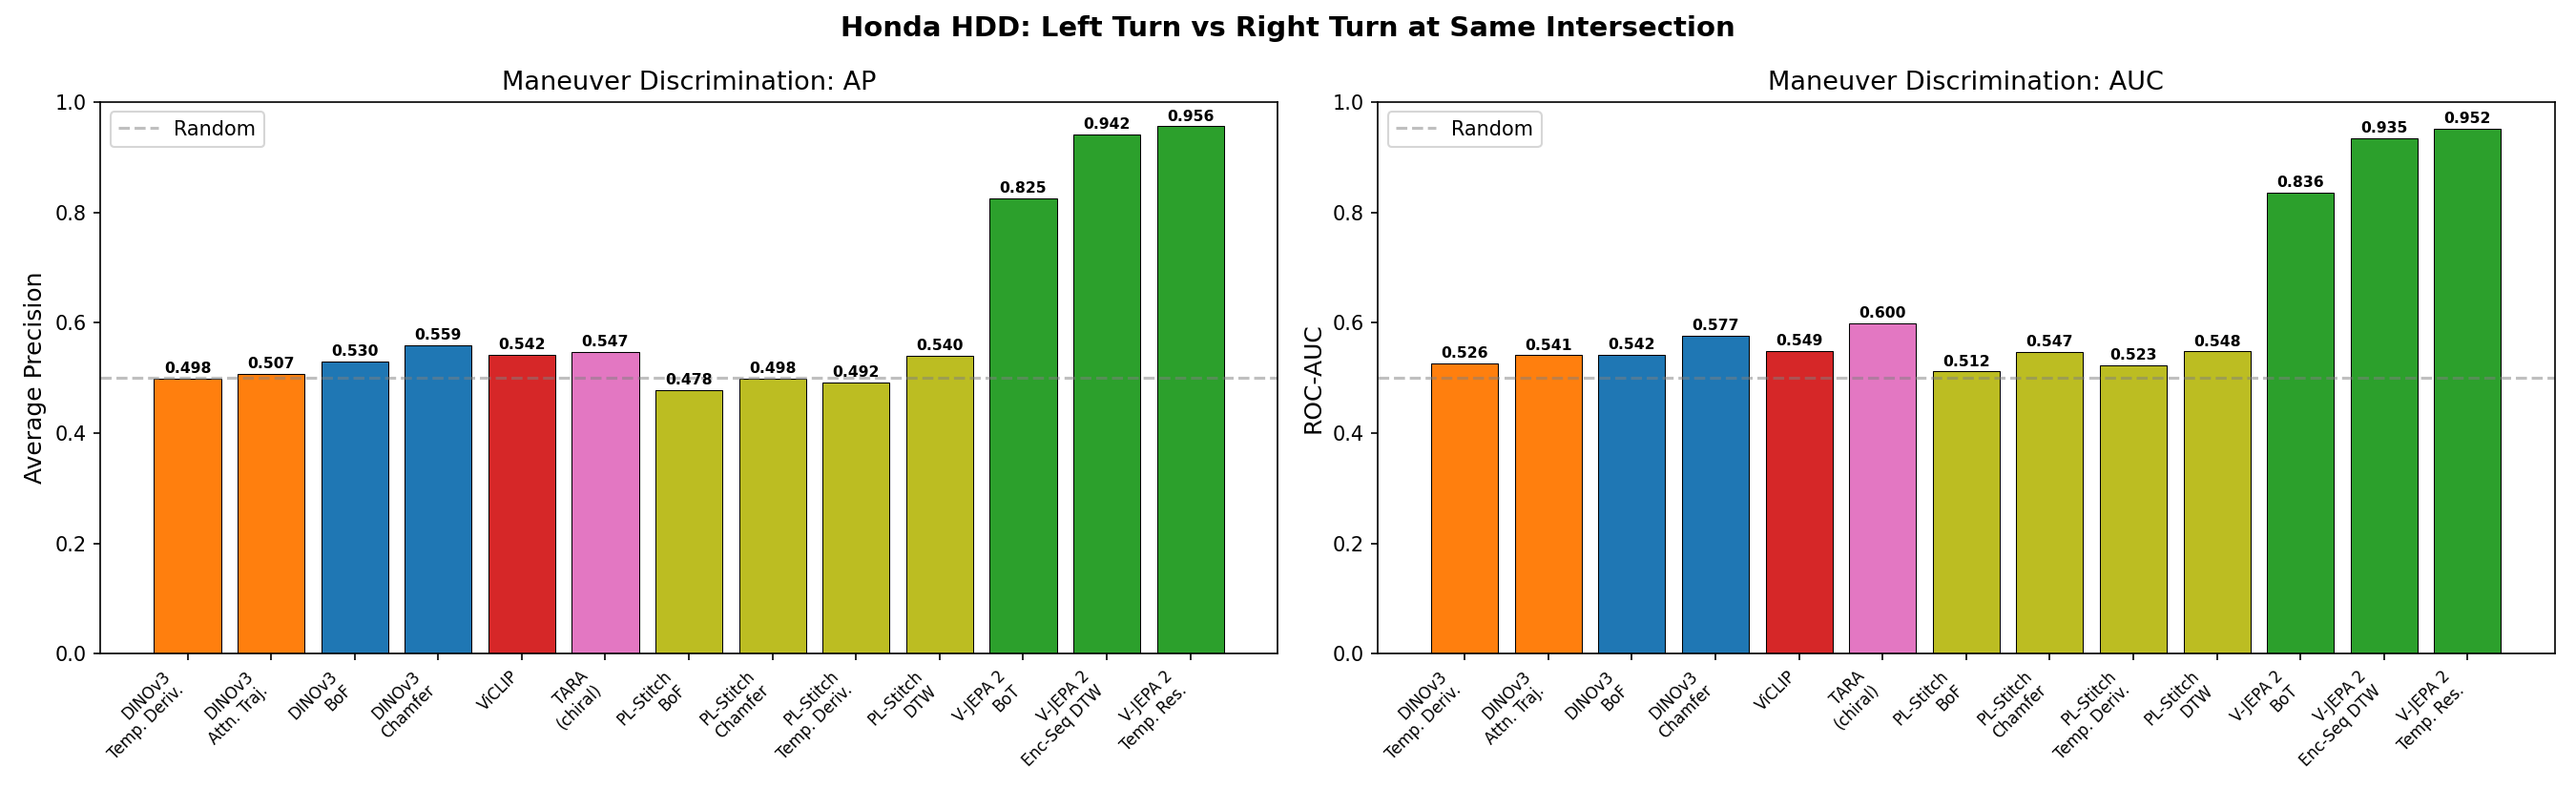
\includegraphics[width=0.60\textwidth]{../figures/hdd_maneuver_discrimination.png}
    \caption{Pooled pair-classification AP on HDD. For V-JEPA~2, BoT $0.825 \to$ Chamfer $0.914 \to$ encoder-sequence DTW $0.942 \to$ temporal residual $0.956$; the 89\% value is a descriptive fraction of this observed AP gap.}
    \label{fig:hdd_maneuver}
    \vspace{-1.2em}
\end{figure}

DINOv3 methods are near chance under this protocol. V-JEPA~2 temporal residuals achieve AP\,=\,0.956; a pixel-difference motion proxy has Spearman $r = 0.051$ (Appendix~\ref{sec:hdd_leakage}), and optical flow (RAFT) achieves AP\,=\,0.478. These controls make a simple intensity explanation unlikely but do not identify the mechanism. Restricting to left-vs-right pairs yields AP\,=\,0.960 [0.958, 0.963] under pair resampling.

Encoder-sequence DTW reaches AP\,=\,0.942. Descriptively, the switch from pooled cosine to per-frame DTW closes 89\% of the observed BoT-to-residual AP gap (0.825$\to$0.956). A paired intersection-cluster bootstrap estimates encoder-sequence DTW minus BoT at $+0.117$ [0.044, 0.127]; residual DTW minus encoder-sequence DTW is $+0.015$ [0.0004, 0.034] (Appendix~\ref{sec:bootstrap_cis}). Symmetric-max aggregation~\cite{kordopatis2019visil} on the same encoder-sequence patches reaches AP\,=\,0.914. Comparing these observed point estimates, Chamfer closes 76\% of the BoT$\to$encoder-sequence-DTW gap; this contrast does not uniquely attribute the remainder to DTW's monotonicity because the comparators differ in more than that constraint.

\textbf{Diagnostic-protocol stress test: does the decomposition compose into a fast retriever?} We evaluate an indexable BoT first stage followed by encoder-sequence-DTW reranking. The corrected protocol is directed and query-wise: every cached HDD segment is a gallery candidate; relevance requires the same GPS cluster and maneuver label; candidates outside the query's cluster remain negatives; and truncated AP@$k$ is normalized by the query's total number of relevant items. The result reverses the conditional pair ranking: full-gallery BoT reaches macro AP\,=\,0.256, while full-gallery encoder-sequence DTW reaches 0.177. At every $k$, DTW reranking reduces both AP and MRR relative to BoT on the same candidate set (Table~\ref{tab:rerank_hdd}; Appendix~\ref{sec:rerank_appendix}). Thus strong discrimination \emph{within a known intersection} does not imply global retrieval once out-of-intersection negatives are restored. A held-out score fusion does not recover the gap either: a per-query linear combination $\alpha\,z(\text{BoT}) + (1{-}\alpha)\,z(-\text{DTW})$ with $\alpha$ chosen by leave-one-cluster-out cross-validation (held-out clusters removed from every tuning query's gallery) selects $\alpha^\star\!=\!0.95$ in all 50 folds and reaches macro AP\,=\,0.257. The paired intersection-cluster difference from BoT is $+0.001$ [$-0.003$, 0.004], providing no detected improvement, while the difference from DTW alone is $+0.080$ [0.064, 0.105].

\begin{table}[ht]
\centering
\caption{Corrected directed HDD retrieval (1{,}673 eligible queries, 50 clusters). Intervals are reported in Appendix~\ref{sec:rerank_appendix}.}
\label{tab:rerank_hdd}
\begin{tabular}{lccc}
\toprule
\textbf{Method} & \textbf{macro AP} & \textbf{recall@$k$} & \textbf{MRR} \\
\midrule
BoT, full gallery & 0.256 & 1.000 & 0.766 \\
Encoder-Seq DTW, full gallery & 0.177 & 1.000 & 0.640 \\
BoT@$100$ & 0.196 & 0.445 & 0.765 \\
\; + DTW rerank@$100$ & 0.144 & 0.445 & 0.657 \\
BoT@$250$ & 0.223 & 0.651 & 0.766 \\
\; + DTW rerank@$250$ & 0.156 & 0.651 & 0.645 \\
\bottomrule
\end{tabular}
\end{table}

TARA~\cite{tara}, a 7B MLLM trained with chiral negatives, has AP\,=\,0.547 under cosine; ViCLIP has 0.542. PL-Stitch~\cite{plstitch} (ViT-Base, Plackett-Luce ranking) supports the same factorial: BoF yields AP\,=\,0.478 and DTW on raw embeddings 0.540. Their similar point estimates should not be called statistically indistinguishable without a paired test. PL-Stitch's low self-reversal $s_\text{rev}\!=\!0.006$ under raw DTW shows that this comparator detects reversal changes, but that property alone does not yield strong maneuver discrimination.

\subsubsection{Sampling Density: Context Window Sweep}
\label{sec:context_sweep}

We fix the backbone and pair set on HDD and sweep context padding $c \in \{1.0, \ldots, 8.0\}$ seconds before and after each maneuver, always extracting 64 unique frames. The actual clip duration is the maneuver duration plus $2c$, so $c$ is not itself the clip duration or the denominator of an exact effective-frame-rate calculation. V-JEPA~2 temporal residual degrades more slowly than BoT as context widens; the observed residual-vs-BoT gap grows from $+0.038$ at $c\!=\!1$\,s to $+0.224$ at $c\!=\!8$\,s (Appendix~\ref{sec:context_sweep_table}).

\subsubsection{Cross-Dataset Validation: nuScenes}
\label{sec:nuscenes}

To test whether the ranking transfers, we evaluate on nuScenes~\cite{nuscenes}. Turn labels come from CAN bus, and intersections are clustered via DBSCAN ($\epsilon\!=\!30$m), yielding 264 segments across 50 mixed-direction clusters (950 pairs).

V-JEPA~2 encoder-sequence DTW reaches AP\,=\,0.867, ahead of the temporal residual (0.815) and BoT (0.791), while DINOv3 methods are at $\leq$0.623. Paired intersection-cluster bootstrap differences support encoder-sequence DTW over BoT ($+0.075$ [0.029, 0.128]) and over the residual ($+0.052$ [0.036, 0.064]). The residual--BoT contrast is less certain ($+0.024$ [$-0.031$, 0.090]). Differences in native sampling are one possible explanation, not an identified cause.

\subsubsection{Cross-Domain Validation: Something-Something V2}
\label{sec:ssv2}

Something-Something V2~\cite{ssv2} is a non-driving cross-domain test: tabletop manipulation with chiral template pairs (Section~\ref{sec:methods}; 400 clips, four pairs, 50 per template). DINOv3 attention-trajectory DTW achieves AP\,=\,0.720, the strongest result; V-JEPA~2 temporal residual (0.556) and BoT (0.555) show only modest transfer from ego-motion driving, and all DINOv3 pooled methods sit at chance (AP\,=\,0.500). The split (attention trajectories on tabletop scenes vs.\ residuals on driving) is interpreted alongside HDD and nuScenes in Section~\ref{sec:discussion}.

\subsection{VLM Prompt and Readout Dependence (EPIC-Kitchens)}

Prior work documents weak temporal performance in VLM generative QA~\cite{tomato,temporalbench,tempcompass,infact,videozerobench}. We extend the analysis to \emph{retrieval embeddings} and compare readouts rather than assuming signal absence. We evaluate three VLMs on 500 EPIC-Kitchens-100~\cite{epickitchens} sequences: Qwen3-VL-8B, Gemma-4-31B, and LLaVA-Video-7B (preliminary VCDB results appear in Appendix~\ref{sec:qwen_vcdb}).

\subsubsection{Generative Probes}
\label{sec:vlm_generative}

Each model received identical frames with three semantically equivalent prompts asking to classify temporal direction.

\begin{table}[ht]
\centering
\caption{Direct direction-prompt classification on EPIC-Kitchens (500 sequences for open-weight models, 200 for API models). Metric and $\pm$ convention defined in \S\ref{sec:methods}; $\pm$ values are prompt-sensitivity SD, not statistical uncertainty.}
\label{tab:vlm_generative}
\begin{tabular}{lcccc}
\toprule
\textbf{Model} & \textbf{Prompt 0} & \textbf{Prompt 1} & \textbf{Prompt 2} & \textbf{Mean Bal.\ Acc.} \\
\midrule
Qwen3-VL-8B & 0.517 & 0.502 & 0.504 & $0.508 \pm 0.007$ \\
Gemma-4-31B & 0.549 & 0.528 & 0.535 & $0.538 \pm 0.009$ \\
LLaVA-Video-7B & 0.503 & 0.501 & 0.505 & $0.503 \pm 0.002$ \\
\midrule
Claude Opus 4.6~\cite{claude4opus} & 0.490 & 0.590 & 0.555 & $0.545 \pm 0.055$ \\
Gemini 3.1 Pro & 0.585 & 0.608 & 0.603 & $0.599 \pm 0.010$ \\
\bottomrule
\end{tabular}
\end{table}

Under these direct prompts, the open-weight models are near chance and Gemini~3.1 Pro~\cite{gemini31pro} reaches $0.599 \pm 0.010$. This is not evidence that the outputs contain no temporal information: an intact-vs.-tampered integrity prompt on the same clips reaches balanced accuracy 0.879 for Qwen3-VL and 0.845 for Gemma-4 (Appendix~\ref{sec:integrity_probe}). Together with strong answer-prior changes across prompt phrasings (Appendix~\ref{sec:prompt_details}), the result demonstrates prompt- and readout-dependence.

\subsubsection{Embedding Probes Across Readouts}
\label{sec:vlm_embedding}

Direct direction prompts are weak. We next probe how forward/reverse changes appear under fixed comparisons of internal representations.

\begin{table}[ht]
\centering
\caption{Comparator-specific $s_\text{rev}$ across the VLM pipeline on EPIC-Kitchens (500 sequences), with pair-bootstrap intervals where available. Cosine and DTW rows use different scales and are not ranked against each other. DINOv3 fingerprints are shown for reference.$^*$}
\label{tab:vlm_embedding}
\begin{tabular}{lc}
\toprule
\textbf{Method} & $s_\text{rev}$ \textbf{[95\% CI]} \\
\midrule
\multicolumn{2}{l}{\emph{DINOv3 structural fingerprints (reference)}} \\
\quad BoF & 1.000 \\
\quad Chamfer & 0.9999 \\
\quad Temporal Derivative & 0.500 [0.499, 0.500] \\
\quad Attention Trajectory & 0.192 [0.187, 0.197] \\
\midrule
\multicolumn{2}{l}{\emph{V-JEPA 2}} \\
\quad BoT (cosine) & 0.9835 [0.9824, 0.9844] \\
\quad Temporal Residual (DTW) & 0.0033 [0.0031, 0.0034] \\
\midrule
\multicolumn{2}{l}{\emph{VLM vision towers (pooled)}} \\
\quad Gemma-4 (SigLIP) & 1.000$^\dagger$ \\
\quad LLaVA (CLIP) & 1.000$^\dagger$ \\
\midrule
\multicolumn{2}{l}{\emph{VLM vision sequence (per-frame DTW)}} \\
\quad Gemma-4 (SigLIP) & 0.492 [0.491, 0.493] \\
\quad LLaVA (CLIP) & 0.495 [0.495, 0.496] \\
\midrule
\multicolumn{2}{l}{\emph{VLM LLM hidden state}} \\
\quad Gemma-4 (Gemma) & 1.000 [1.000, 1.000] \\
\quad LLaVA (Qwen2) & 0.998 [0.998, 0.999] \\
\quad Qwen3-VL (Qwen3) & 0.998 [0.998, 0.999] \\
\bottomrule
\end{tabular}
\begin{flushleft}
\small $^*$DINOv3 300M params, CLIP (ViT-L) 304M, SigLIP (SO-400M) 400M. Exact invariance follows only when a symmetric comparator receives fixed independently encoded elements; pooled contextual values are empirical. $^\dagger$Raw values 1.001--1.002 from f32 precision; clamped to 1.000. We omit Qwen3-VL vision probes from this table because its ViT uses dynamic-resolution spatial grids with 3D temporal--spatial merging, which disrupts clean per-frame token grouping for the detailed $s_\text{rev}$ analysis; approximate pooled and sequence results appear in Table~\ref{tab:summary_vlm}. The LLM hidden-state probe is unaffected.
\end{flushleft}
\end{table}

\textbf{Sequence comparisons expose changes that pooling suppresses.} Pooled VLM vision embeddings have cosine $s_\text{rev} \approx 1.0$, while retaining per-frame tokens and comparing their derivatives via DTW gives substantially lower values on that comparator's separate scale. V-JEPA~2 shows the same readout dependence particularly strongly: BoT cosine is 0.9835, whereas temporal-residual DTW is 0.0033. Mean-pooled LLM readouts similarly have $s_\text{rev} \approx 1.0$ across layers (Appendix~\ref{sec:layer_ablation}), while per-position hidden states change enough for sequence DTW to detect (Appendix~\ref{sec:vision_token_probe}). The current fixed-dimensional learned probes do not provide reliable evidence of direction decoding (best observed accuracy 0.560 across many configurations; Appendix~\ref{sec:linear_probe}), but this exploratory multiple-comparison result is not a proof of absence.

\subsection{Cross-Method Summary}

Full cross-method comparisons across the seven benchmarks are in Appendix~\ref{sec:cross_method_tables} (Tables~\ref{tab:summary_encoders} and~\ref{tab:summary_vlm}). No evaluated method has the best observed point estimate in every regime: Chamfer is strongest on VCDB (AP\,=\,0.989), V-JEPA~2 temporal residual is strongest on the HDD pair diagnostic (AP\,=\,0.956), and DINOv3 attention trajectories are strongest on the selected SSv2 split (AP\,=\,0.720). VLM conclusions depend on the prompt and readout.

\section{Related Work}
\label{sec:related_work}

\textbf{Video copy detection.} Standard benchmarks (ISC~\cite{douze2021isc}, VSC~\cite{pizzi2023vsc}, VCSL~\cite{he2022vcsl}) and descriptors (SSCD~\cite{pizzi2022sscd}, ViSiL~\cite{kordopatis2019visil}, DnS~\cite{kordopatis2022dns}, S2VS~\cite{s2vs}) provide per-frame features with learned aggregation. Wang et al.~\cite{wang2023duallevel} win the Meta VSC challenge; subsequent analysis~\cite{fojcik2025} exposes temporal-attack vulnerability. Explicit temporal alignment (VSAL~\cite{han2021vsal}, TransVCL~\cite{he2023transvcl}) shows order matters for copy localization. We diagnose \emph{when} temporal structure helps versus hurts.

\textbf{Temporal sensitivity in video models.} Lei et al.~\cite{lei2022singleframe} established the static-bias problem. Subsequent work diagnoses this in \emph{generative} VLM QA~\cite{tempcompass,bagad2023testtime,temporalbench,vbenchcomp,tomato}, including recent hallucination and zero-shot benchmarks~\cite{infact,videozerobench}. Most closely, concurrent work traces arrow-of-time information through the vision encoder, projector, and language model and intervenes on the projector~\cite{tracingaot}; our VLM localization is therefore corroborative rather than the primary novelty. Other arrow-of-time diagnostics~\cite{aot,arrowrl} and studies~\cite{timeblindness,timeblind,vitatecs,reveal,weavetime} further narrow the novelty of a blanket temporal-blindness claim. Our distinct focus is retrieval evaluation and executable comparator diagnostics. NExT-GQA~\cite{nextgqa} introduces $\mathrm{GQ}@\tau$, a joint grounded-QA metric complementary to the pooled pair AP we report. \emph{Training-time} fixes are complementary: TGPO's~\cite{tgpo} binary ordered/shuffled reward relates to our continuous $K$-gradient; PL-Stitch~\cite{plstitch} and ArrowGEV~\cite{arrowgev} inject pretraining order sensitivity; TARA~\cite{tara} trains with chiral negatives.

\textbf{Video prediction for temporal understanding.} V-JEPA~2~\cite{vjepa2} learns spatiotemporal representations via masked prediction. Drive-JEPA~\cite{drivejepa} is a downstream application (JEPA distillation for end-to-end driving), not a competing diagnosis; we instead treat V-JEPA~2 as one of several encoders under a retrieval-diagnosis lens. TWLV-I~\cite{twlvi} evaluates appearance vs.\ motion across video foundation models. Li et al.~\cite{temporaltransfer} show temporal information is encoded but standard pipelines fail to surface it, matching our finding.

\textbf{Temporal alignment for retrieval.} DTW~\cite{sakoe1978dtw} remains standard; extensions include Soft-DTW~\cite{ddtw} and Drop-DTW~\cite{dropdtw}. We use DTW as a diagnostic tool; Weller et al.~\cite{weller2025limits} provide theoretical justification for multi-vector approaches.

\section{Discussion}
\label{sec:discussion}

\textbf{Scene matching} (VCDB, Nymeria, MUVR). BoF wins; temporal methods add noise (Appendix~\ref{sec:scene_matching}). Order-invariance is a feature here, not a bug.

\textbf{Motion dynamics} (HDD, nuScenes, SSv2). The best observed representation--comparator combination is domain-dependent: V-JEPA~2 variants have the strongest HDD and nuScenes conditional pair results, while attention trajectories lead on the selected SSv2 split. Paired cluster contrasts support encoder-sequence DTW over BoT on both driving datasets. However, the corrected global HDD gallery reverses that ranking, showing that conditional pair discrimination and end-to-end retrieval test different capabilities. Temporal-training controls (TARA~\cite{tara}, PL-Stitch~\cite{plstitch}, ViCLIP~\cite{viclip}, X-CLIP~\cite{xclip}) do not lead these evaluations.

\textbf{Temporal manipulation} (reversal, scrambling). Exact invariance applies to fixed independently encoded frame sets under symmetric comparison. Contextual video encoders and VLMs instead show probe-dependent sensitivity: sequence comparisons detect changes, direct direction prompts are weak, and integrity prompts are substantially stronger. These outcomes should not be collapsed into one cross-comparator $s_\text{rev}$ ranking.

\textbf{Architecture implications.} Symmetric aggregation over independently encoded elements guarantees invariance; contextual encoding can retain temporal effects before pooling. The HDD query-wise result also shows that replacing the comparator after an appearance-based candidate stage is insufficient: the temporal score must retain global location discrimination. A held-out linear fusion with the first-stage BoT score does not remedy this on our gallery---cross-validated weights collapse onto BoT ($\alpha^\star\!\to\!0.95$) with no detected gain---so recovering global retrieval requires a temporal representation that is itself location-discriminative, not merely a better ranking rule over the existing scores.

\textbf{World model implications.} V-JEPA~2's results are consistent with its predictive objective~\cite{lecun_worldmodel,vjepa2}, but these experiments do not isolate that objective as the cause. Concurrent interpretability~\cite{joseph2026physics} localizes physics representations to an intermediate-depth V-JEPA~2 transition with distributed directional encoding, consistent with temporal effects surviving in the backbone but requiring task-specific readouts.

\begin{algorithm}[h]
\caption{Temporal Sensitivity Diagnostic Protocol}
\label{alg:decision}
\begin{algorithmic}[1]
\State Run \emph{scramble gradient}. A flat curve means no sensitivity was detected under this intervention.
\State Run the feature--comparator factorial on one shared pair set; report controlled contrasts without causal language.
\State Run \emph{sampling-density sweep}; isolate frame-rate / context-window effects.
\State Use paired group-level bootstrap where groups exist; compare generative and embedding probes without treating disagreement as a unique causal diagnosis.
\end{algorithmic}
\end{algorithm}

\textbf{Limitations.} DTW is not indexable ($O(T^2)$); probes train on 400 samples in $p \gg n$ and explore many configurations without a held-out selection protocol; ViCLIP's 8-frame input confounds comparison with 64-frame V-JEPA~2; most AP results pool dependent pairs that share clips, so pair-bootstrap intervals are descriptive and cluster-level inference is required where grouping is available; and the selected SSv2 split is small. The results establish diagnostic behavior on these datasets, not a universal architecture ranking.


\section{Conclusion}

We introduced executable diagnostics for locating temporal sensitivity in video-retrieval pipelines. Exact invariance is confined to symmetric comparisons of fixed element representations; contextual encoders, comparator choice, prompt, and readout all affect the empirical outcome. Paired cluster contrasts support comparator effects on the conditional HDD and nuScenes pair tasks, while corrected directed retrieval shows that the same DTW score underperforms BoT in a global gallery. Temporal sensitivity is therefore necessary for some motion queries but not sufficient for retrieval: evaluation must test both the intended conditional distinction and the full candidate distribution.\footnote{Toolkit code: \url{https://anonymous.4open.science/r/video-temporal-diagnostics-F450}.}

\FloatBarrier  % Force all main-body floats before references

\begin{thebibliography}{99}
\bibitem{vjepa2} M.~Assran, A.~Bardes, D.~Fan, Q.~Garrido et al. V-JEPA~2: Self-Supervised Video Models Enable Understanding, Prediction and Planning. \emph{arXiv:2506.09985}, 2025.
\bibitem{dinov3} O.~Sim\'{e}oni, H.~V.~Vo, M.~Seitzer, F.~Baldassarre et al. DINOv3. \emph{arXiv:2508.10104}, 2025.
\bibitem{vcdb} Y.-G.~Jiang, Y.~Jiang, J.~Liu, Z.~Chen. VCDB: A Large-Scale Database for Partial Copy Detection in Videos. In \emph{ECCV}, 2014.
\bibitem{honda_hdd} V.~Ramanishka, Y.-T.~Chen, T.~Misu, K.~Saenko. Toward Driving Scene Understanding: A Dataset for Learning Driver Behavior and Causal Reasoning. In \emph{CVPR}, 2018.
\bibitem{nuscenes} H.~Caesar et al. nuScenes: A multimodal dataset for autonomous driving. In \emph{CVPR}, 2020.
\bibitem{epickitchens} D.~Damen, H.~Doughty, G.~M.~Farinella, A.~Furnari et al. Rescaling Egocentric Vision: Collection, Pipeline and Challenges for EPIC-KITCHENS-100. \emph{IJCV}, 130(1):33--55, 2022.
\bibitem{ssv2} R.~Goyal, S.~Ebrahimi~Kahou, V.~Michalski, J.~Materzy\'nska et al. The ``Something Something'' Video Database for Learning and Evaluating Visual Common Sense. In \emph{ICCV}, 2017.
\bibitem{fojcik2025} K.~Fojcik and P.~Syga. Counteracting temporal attacks in video copy detection. \emph{arXiv:2501.11171}, 2025.
\bibitem{3dcsl} R.~Deng, Q.~Wu, Y.~Li. 3D-CSL: self-supervised 3D context similarity learning for Near-Duplicate Video Retrieval. \emph{arXiv:2211.05352}, 2022.
\bibitem{plstitch} C.~Che, C.~Wang, X.~Chen, S.~Tsoka, and L.~C.~Garcia-Peraza-Herrera. A Stitch in Time: Learning Procedural Workflow via Self-Supervised Plackett-Luce Ranking. \emph{arXiv:2511.17805}, 2025.
\bibitem{arrowgev} F.~Yu, Z.~Lu, L.~Niu, F.~Meng. ArrowGEV: Grounding Events in Video via Learning the Arrow of Time. \emph{arXiv:2601.06559}, 2026.
\bibitem{weavetime} Y.~Zhang, C.~Shi, S.~Yang. WeaveTime: Stream from Earlier Frames into Emergent Memory in VideoLLMs. \emph{arXiv:2602.22142}, 2026.
\bibitem{tracingaot} P.~Han, F.~Cheng, L.~K.~Pereira et al. Tracing the Arrow of Time: Diagnosing Temporal Information Flow in Video-LLMs. \emph{arXiv:2605.07568}, 2026.
\bibitem{timeblindness} U.~Upadhyay et al. Time Blindness: Why Video-Language Models Can't See What Humans Can? \emph{arXiv:2505.24867}, 2025.
\bibitem{qwen3vl} Qwen Team. Qwen3-VL Technical Report. \emph{arXiv:2511.21631}, 2025.
\bibitem{gemma4} Google DeepMind. Gemma~4 Model Card. \url{https://ai.google.dev/gemma/docs/core/model_card_4}, 2026.
\bibitem{llavavideo} Y.~Zhang et al. LLaVA-Video: Video Instruction Tuning With Synthetic Data. \emph{arXiv:2410.02713}, 2024.
\bibitem{aot} S.~Matta, L.~K.~Pereira, P.~Han, F.~Cheng. Which Way Does Time Flow? A Psychophysics-Grounded Evaluation for Vision-Language Models. \emph{arXiv:2510.26241}, 2025.
\bibitem{vitatecs} S.~Li et al. VITATECS: A Diagnostic Dataset for Temporal Concept Understanding of Video-Language Models. In \emph{ECCV}, 2024.
\bibitem{muvr} Y.~Feng et al. MUVR: A Multi-Modal Untrimmed Video Retrieval Benchmark with Multi-Level Visual Correspondence. \emph{arXiv:2510.21406}, 2025.
\bibitem{semdedup} A.~Abbas et al. SemDeDup: Data-efficient learning at web-scale through semantic deduplication. \emph{arXiv:2303.09540}, 2023.
\bibitem{faiss} J.~Johnson et al. Billion-scale similarity search with GPUs. \emph{IEEE Transactions on Big Data}, 2019.
\bibitem{ddtw} M.~Cuturi and M.~Blondel. Soft-{DTW}: a Differentiable Loss Function for Time-Series. In \emph{ICML}, 2017.
\bibitem{douze2021isc} M.~Douze, G.~Tolias, E.~Pizzi et al. The 2021 Image Similarity Dataset and Challenge. In \emph{NeurIPS Competition Track}, 2021.
\bibitem{pizzi2023vsc} E.~Pizzi, G.~Kordopatis-Zilos, H.~Patel, G.~Postelnicu et al. The 2023 Video Similarity Dataset and Challenge. \emph{Computer Vision and Image Understanding}, 2024.
\bibitem{pizzi2022sscd} E.~Pizzi, S.~D.~Roy, S.~N.~Ravindra, P.~Goyal, and M.~Douze. A Self-Supervised Descriptor for Image Copy Detection. In \emph{CVPR}, 2022.
\bibitem{kordopatis2019visil} G.~Kordopatis-Zilos, S.~Papadopoulos, I.~Patras, and I.~Kompatsiaris. ViSiL: Fine-grained Spatio-Temporal Video Similarity Learning. In \emph{ICCV}, 2019.
\bibitem{kordopatis2022dns} G.~Kordopatis-Zilos, C.~Tzelepis, S.~Papadopoulos, I.~Kompatsiaris, and I.~Patras. DnS: Distill-and-Select for Efficient and Accurate Video Indexing and Retrieval. \emph{IJCV}, 2022.
\bibitem{he2022vcsl} S.~He et al. A Large-scale Comprehensive Dataset and Copy-overlap Aware Evaluation Protocol for Segment-level Video Copy Detection. In \emph{CVPR}, 2022.
\bibitem{he2023transvcl} S.~He et al. TransVCL: Attention-enhanced Video Copy Localization Network with Flexible Supervision. In \emph{AAAI}, 2023.
\bibitem{han2021vsal} Z.~Han, X.~He, M.~Tang, and Y.~Lv. Video Similarity and Alignment Learning on Partial Video Copy Detection. In \emph{ACM~MM}, 2021.
\bibitem{sakoe1978dtw} H.~Sakoe and S.~Chiba. Dynamic Programming Algorithm Optimization for Spoken Word Recognition. \emph{IEEE Trans.\ Acoustics, Speech, and Signal Processing}, 26(1):43--49, 1978.
\bibitem{nymeria} L.~Ma et al. Nymeria: A Massive Collection of Multimodal Egocentric Daily Motion in the Wild. In \emph{ECCV}, 2024.
\bibitem{reveal} T.~V.~Sethuraman et al. Stress Tests REVEAL Fragile Temporal and Visual Grounding in Video-Language Models. \emph{arXiv:2602.11244}, 2026.
\bibitem{timeblind} B.~Li et al. TimeBlind: A Spatio-Temporal Compositionality Benchmark for Video LLMs. \emph{arXiv:2602.00288}, 2026.
\bibitem{tgpo} Z.~Xu et al. Incentivizing Temporal-Awareness in Egocentric Video Understanding Models. \emph{arXiv:2603.27184}, 2026.
\bibitem{tara} P.~Bagad and A.~Zisserman. TARA: Simple and Efficient Time Aware Retrieval Adaptation of MLLMs for Video Understanding. \emph{arXiv:2512.13511}, 2025.
\bibitem{drivejepa} L.~Wang et al. Drive-JEPA: Video JEPA Meets Multimodal Trajectory Distillation for End-to-End Driving. \emph{arXiv:2601.22032}, 2026.
\bibitem{weller2025limits} O.~Weller, M.~Boratko, I.~Naim, and J.~Lee. On the Theoretical Limitations of Embedding-Based Retrieval. \emph{arXiv:2508.21038}, 2025.
\bibitem{nextgqa} J.~Xiao, A.~Yao, Y.~Li, and T.-S.~Chua. Can I Trust Your Answer? Visually Grounded Video Question Answering. In \emph{CVPR}, 2024. \emph{arXiv:2309.01327}.
\bibitem{lei2022singleframe} J.~Lei, T.~L.~Berg, and M.~Bansal. Revealing Single Frame Bias for Video-and-Language Learning. In \emph{ACL}, 2023.
\bibitem{bagad2023testtime} P.~Bagad, M.~Tapaswi, and C.~G.~M.~Snoek. Test of Time: Instilling Video-Language Models with a Sense of Time. In \emph{CVPR}, 2023.
\bibitem{tempcompass} Y.~Liu, S.~Li, Y.~Liu et al. TempCompass: Do Video LLMs Really Understand Videos? \emph{arXiv:2403.00476}, 2024.
\bibitem{twlvi} H.~Lee, J.-Y.~Kim, K.~Baek et al. TWLV-I: Analysis and Insights from Holistic Evaluation on Video Foundation Models. \emph{arXiv:2408.11318}, 2024.
\bibitem{temporaltransfer} L.~Li, Y.~Liu, L.~Yao et al. Temporal Reasoning Transfer from Text to Video. In \emph{ICLR}, 2025.
\bibitem{tomato} Z.~Shangguan, C.~Li, Y.~Ding et al. TOMATO: Assessing Visual Temporal Reasoning Capabilities in Multimodal Foundation Models. In \emph{ICLR}, 2025.
\bibitem{temporalbench} M.~Cai, R.~Tan, J.~Zhang et al. TemporalBench: Benchmarking Fine-grained Temporal Understanding for Multimodal Video Models. \emph{arXiv:2410.10818}, 2024.
\bibitem{s2vs} G.~Kordopatis-Zilos, G.~Tolias, C.~Tzelepis, I.~Kompatsiaris, I.~Patras, and S.~Papadopoulos. Self-Supervised Video Similarity Learning. \emph{arXiv:2304.03378}, 2023.
\bibitem{arrowrl} Z.~Xue, M.~Luo, and K.~Grauman. Seeing the Arrow of Time in Large Multimodal Models. In \emph{NeurIPS}, 2025. \emph{arXiv:2506.03340}.
\bibitem{dropdtw} N.~Dvornik, I.~Hadji, K.~G.~Derpanis, and A.~Garg. Drop-DTW: Aligning Common Signal Between Sequences While Dropping Outliers. In \emph{NeurIPS}, 2021.
\bibitem{vbenchcomp} B.~Feng, Z.~Lai, S.~Li, Z.~Wang, S.~Wang, P.~Huang, and M.~Cao. Breaking Down Video LLM Benchmarks: Knowledge, Spatial Perception, or True Temporal Understanding? \emph{arXiv:2505.14321}, 2025.
\bibitem{wang2023duallevel} T.~Wang, F.~Ma, Z.~Liu, and F.~Rao. A Dual-Level Detection Method for Video Copy Detection. \emph{arXiv:2305.12361}, 2023.
\bibitem{infact} J.~Yang, Y.~Min, J.~Zhang, S.~Shan, and X.~Chen. INFACT: A Diagnostic Benchmark for Induced Faithfulness and Factuality Hallucinations in Video-LLMs. \emph{arXiv:2603.11481}, 2026.
\bibitem{videozerobench} J.~Meng et al. VideoZeroBench: Probing the Limits of Video MLLMs with Spatio-Temporal Evidence Verification. \emph{arXiv:2604.01569}, 2026.
\bibitem{claude4opus} Anthropic. Claude Opus 4.6 Model Card. \url{https://docs.anthropic.com/en/docs/about-claude/models}, 2026.
\bibitem{gemini31pro} Google DeepMind. Gemini 3.1 Pro. \url{https://ai.google.dev/gemini-api/docs/models}, 2026.
\bibitem{viclip} Y.~Wang, Y.~He, Y.~Li, K.~Li et al. InternVid: A Large-scale Video-Text Dataset for Multimodal Understanding and Generation. In \emph{ICLR}, 2024.
\bibitem{xclip} B.~Ni, H.~Peng, M.~Chen et al. Expanding Language-Image Pretrained Models for General Video Recognition. In \emph{ECCV}, 2022.
\bibitem{deepsets} M.~Zaheer, S.~Kottur, S.~Ravanbakhsh, B.~P\'{o}czos, R.~Salakhutdinov, and A.~Smola. Deep Sets. In \emph{NeurIPS}, 2017.
\bibitem{lecun_worldmodel} Y.~LeCun. A Path Towards Autonomous Machine Intelligence. OpenReview preprint, version~0.9.2, 2022.
\bibitem{tuna} M.~Zhang, Y.~Liu, J.~Lin et al. TUNA: Towards Unified Understanding and Generation in Autoregressive Video Models. In \emph{CVPR}, 2026.
\bibitem{joseph2026physics} S.~Joseph, Q.~Garrido, M.~Kowal, T.~Fel, S.~Bakhtiari, B.~Richards, and M.~Rabbat. Interpreting Physics in Video World Models. \emph{arXiv:2602.07050}, 2026.
\end{thebibliography}

% NeurIPS requires the checklist before the appendix.
\newpage
\section*{NeurIPS Paper Checklist}

\begin{enumerate}

\item {\bf Claims}
    \item[] Question: Do the main claims made in the abstract and introduction accurately reflect the paper's contributions and scope?
    \item[] Answer: \answerYes{}
    \item[] Justification: The abstract distinguishes exact invariance of fixed independently encoded elements from empirical behavior of contextual representations, identifies pair-classification results as diagnostics, and avoids causal attribution. Results invalidated by implementation or protocol changes are marked pending rerun.

\item {\bf Limitations}
    \item[] Question: Does the paper discuss the limitations of the work performed by the authors?
    \item[] Answer: \answerYes{}
    \item[] Justification: Section~5 discusses DTW scalability, probe multiplicity, frame-count confounds, dependent-pair evaluation, the small selected SSv2 split, and limits on cross-dataset generalization.

\item {\bf Theory assumptions and proofs}
    \item[] Question: For each theoretical result, does the paper provide the full set of assumptions and a complete (and correct) proof?
    \item[] Answer: \answerNA{}
    \item[] Justification: The paper makes no new formal theorem claim. The stated permutation invariance of a symmetric function over fixed inputs follows from its definition, and its limited assumptions are made explicit.

    \item {\bf Experimental result reproducibility}
    \item[] Question: Does the paper fully disclose all the information needed to reproduce the main experimental results of the paper to the extent that it affects the main claims and/or conclusions of the paper (regardless of whether the code and data are provided or not)?
    \item[] Answer: \answerNo{}
    \item[] Justification: The code and guide specify the current protocols, but corrected scramble, EPIC residual, paired-bootstrap, and directed-reranking results are pending. Exact feature caches and a locked environment are not included. This answer should be revisited after the documented cluster jobs complete.

\item {\bf Open access to data and code}
    \item[] Question: Does the paper provide open access to the data and code, with sufficient instructions to faithfully reproduce the main experimental results, as described in supplemental material?
    \item[] Answer: \answerNo{}
    \item[] Justification: Code and instructions are provided, but several datasets require separate licenses or access agreements (notably Honda HDD), model weights have their own terms, and feature caches are not redistributed. The guide documents these requirements.

\item {\bf Experimental setting/details}
    \item[] Question: Does the paper specify all the training and test details (e.g., data splits, hyperparameters, how they were chosen, type of optimizer) necessary to understand the results?
    \item[] Answer: \answerYes{}
    \item[] Justification: No training is performed; all experiments use frozen pretrained models. Evaluation details (pair construction, DBSCAN $\epsilon$, negative-sampling ratios, bootstrap parameters, DTW $\alpha$ values, frame counts) are specified in Sections~2--3 and the appendix.

\item {\bf Experiment statistical significance}
    \item[] Question: Does the paper report error bars suitably and correctly defined or other appropriate information about the statistical significance of the experiments?
    \item[] Answer: \answerNo{}
    \item[] Justification: Existing pair-resampling intervals are now labeled descriptive because pairs share clips. HDD and nuScenes require paired cluster-bootstrap contrasts, and analogous independent-unit analyses are not yet available for every benchmark. Prompt standard deviations measure prompt sensitivity, not sampling uncertainty.

\item {\bf Experiments compute resources}
    \item[] Question: For each experiment, does the paper provide sufficient information on the computer resources (type of compute workers, memory, time of execution) needed to reproduce the experiments?
    \item[] Answer: \answerNo{}
    \item[] Justification: The paper reports the GPU class and approximate microbenchmarks, but it does not yet provide measured wall time and peak memory for every experiment. The supplied SLURM jobs provide requested resources for the corrected runs.

\item {\bf Code of ethics}
    \item[] Question: Does the research conducted in the paper conform, in every respect, with the NeurIPS Code of Ethics \url{https://neurips.cc/public/EthicsGuidelines}?
    \item[] Answer: \answerYes{}
    \item[] Justification: The research uses only publicly available datasets and pretrained models. The reversal attack analysis in Section~3.1 is diagnostic (identifying a vulnerability in existing systems) rather than offensive.

\item {\bf Broader impacts}
    \item[] Question: Does the paper discuss both potential positive societal impacts and negative societal impacts of the work performed?
    \item[] Answer: \answerYes{}
    \item[] Justification: The paper identifies a concrete Trust \& Safety vulnerability (reversal attack bypassing VCD filters) and diagnoses temporal blindness in video retrieval systems deployed at scale. The diagnostic framework itself poses minimal misuse risk as it characterizes existing model behavior rather than introducing new attack vectors.

\item {\bf Safeguards}
    \item[] Question: Does the paper describe safeguards that have been put in place for responsible release of data or models that have a high risk for misuse (e.g., pre-trained language models, image generators, or scraped datasets)?
    \item[] Answer: \answerNA{}
    \item[] Justification: The paper does not release new models or datasets. It evaluates existing publicly available models on existing public benchmarks.

\item {\bf Licenses for existing assets}
    \item[] Question: Are the creators or original owners of assets (e.g., code, data, models), used in the paper, properly credited and are the license and terms of use explicitly mentioned and properly respected?
    \item[] Answer: \answerYes{}
    \item[] Justification: All datasets and models are cited with their original publications. Appendix~\ref{sec:licenses} lists the governing license for each asset (datasets: VCDB research-only, Honda HDD HRI-USA Data Use Agreement, nuScenes CC BY-NC-SA 4.0, EPIC-Kitchens-100 CC BY-NC 4.0, Nymeria CC BY-NC 4.0, MUVR research-only; model weights listed alongside). All use is non-commercial research, consistent with the most restrictive license.

\item {\bf New assets}
    \item[] Question: Are new assets introduced in the paper well documented and is the documentation provided alongside the assets?
    \item[] Answer: \answerNA{}
    \item[] Justification: The paper does not release new datasets or models.

\item {\bf Crowdsourcing and research with human subjects}
    \item[] Question: For crowdsourcing experiments and research with human subjects, does the paper include the full text of instructions given to participants and screenshots, if applicable, as well as details about compensation (if any)?
    \item[] Answer: \answerNA{}
    \item[] Justification: No crowdsourcing or human subjects research was conducted.

\item {\bf Institutional review board (IRB) approvals or equivalent for research with human subjects}
    \item[] Question: Does the paper describe potential risks incurred by study participants, whether such risks were disclosed to the subjects, and whether Institutional Review Board (IRB) approvals (or an equivalent approval/review based on the requirements of your country or institution) were obtained?
    \item[] Answer: \answerNA{}
    \item[] Justification: No human subjects research was conducted.

\item {\bf Declaration of LLM usage}
    \item[] Question: Does the paper describe the usage of LLMs if it is an important, original, or non-standard component of the core methods in this research? Note that if the LLM is used only for writing, editing, or formatting purposes and does \emph{not} impact the core methodology, scientific rigor, or originality of the research, declaration is not required.
    \item[] Answer: \answerYes{}
    \item[] Justification: Three Video-LLMs (Qwen3-VL, Gemma~4, LLaVA-Video) are evaluated as subjects of the diagnostic study. Their usage is fully described in Sections~2--3. LLMs were also used to assist with writing and code development.

\end{enumerate}


\appendix

\section{FPS Cap Invariance Proof}
\label{sec:fps_invariance}

For V-JEPA~2 on Honda HDD, each clip of duration $d$ seconds is sampled at $\text{target\_fps} = 64 / d$ to fill the 64-frame input. An FPS cap only activates when $\text{target\_fps} > \text{cap}$; otherwise frame selection is identical to the uncapped baseline.

Table~\ref{tab:fps_invariance} confirms that across all 9{,}811 HDD maneuver segments (at $\pm$3\,s context), the maximum $\text{target\_fps}$ is 9.14. Caps at 10, 15, and 30 therefore never activate; the identical AP values at these caps are explained by frame selection invariance, not by a learned robustness plateau.

\begin{table}[h]
\centering
\caption{FPS cap activation across all HDD segments ($\pm$3\,s context). Caps $\geq$10 activate for zero segments, confirming identical frame selection to the uncapped baseline. Unique frames = number of distinct video frames extracted before padding to 64.}
\label{tab:fps_invariance}
\begin{tabular}{rrrrl}
\toprule
FPS Cap & \% Active & Mean Unique & Mean Dup\% & Effect \\
\midrule
2  & 99.9\% & 20.2 & 68.4\% & Strong degradation \\
5  & 85.9\% & 49.1 & 23.3\% & Moderate degradation \\
10 & 0.0\%  & 64.0 & 0.0\%  & No-op (identical to baseline) \\
15 & 0.0\%  & 64.0 & 0.0\%  & No-op (identical to baseline) \\
30 & 0.0\%  & 64.0 & 0.0\%  & No-op (identical to baseline) \\
\bottomrule
\end{tabular}
\end{table}

Segment durations range from 7.0\,s to 46.0\,s (mean 10.1\,s), yielding $\text{target\_fps} \in [1.39, 9.14]$ (mean 6.66). All values fall below the lowest non-trivial cap (10\,FPS), so meaningful degradation occurs only when the cap drops below the native target rate.

\section{VCDB Reversal Attack Figure}
\label{sec:reversal_figure}

Figure~\ref{fig:reversal_attack} visualizes Table~\ref{tab:vcdb_reversal_attack}: AP under forward and reversed playback across five methods on VCDB. Order-invariant methods (BoF, Chamfer, V-JEPA~2 BoT) show no drop; only attention-trajectory DTW exposes the reversal, with the V-JEPA~2 temporal residual showing a partial drop. We move the figure here because the table already carries the same evidence in a denser form.

\begin{figure}[h]
    \centering
    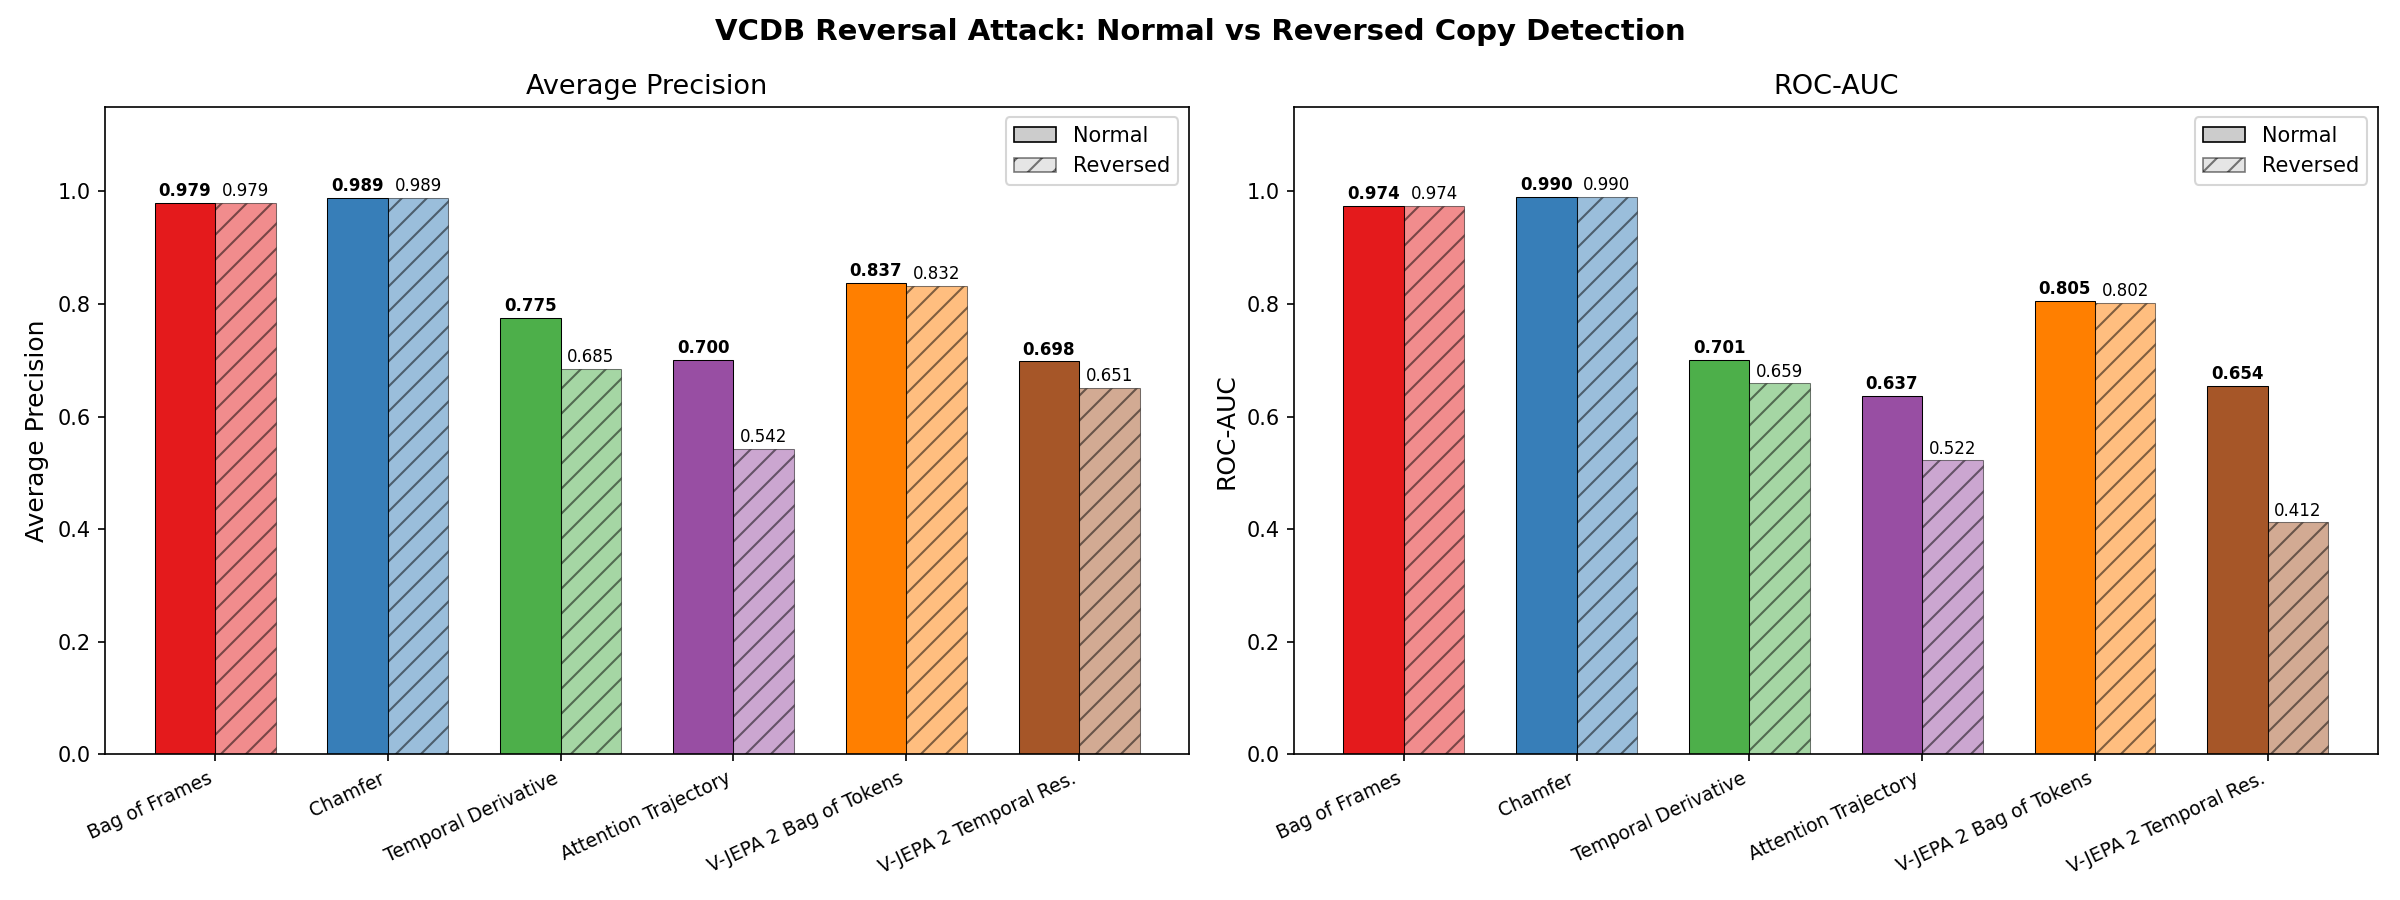
\includegraphics[width=0.9\textwidth]{../figures/vcdb_reversal_attack.png}
    \caption{VCDB Reversal Attack (528 videos, 5{,}585 positive pairs). Order-invariant methods (BoF, Chamfer) maintain identical AP/AUC under reversal. Only sequence-aware methods (Attention Trajectory) register the structural tampering via an AP drop.}
    \label{fig:reversal_attack}
\end{figure}

\section{Context Sweep Table}
\label{sec:context_sweep_table}

Table~\ref{tab:context_sweep} reports the Section~\ref{sec:context_sweep} context experiment. The parameter $c \in \{1.0, 2.0, 3.0, 4.0, 6.5, 8.0\}$ is seconds of padding on each side of a variable-duration maneuver; it is not the final clip duration. We extract 64 unique frames from each resulting window.

\begin{table}[h]
\centering
\caption{Context-padding sweep on HDD (1{,}687 maneuvers, 64 unique frames). The final duration is maneuver duration plus $2c$.}
\label{tab:context_sweep}
\begin{tabular}{rccc}
\toprule
\textbf{context\_sec ($c$)} & \textbf{Temporal Residual AP} & \textbf{BoT AP} & \textbf{$\Delta$ (Res.\ $-$ BoT)} \\
\midrule
1.0 & 0.962 & 0.924 & +0.038 \\
2.0 & 0.963 & 0.877 & +0.086 \\
3.0 & 0.956 & 0.825 & +0.131 \\
4.0 & 0.940 & 0.774 & +0.166 \\
6.5 & 0.872 & 0.663 & +0.209 \\
8.0 & 0.838 & 0.614 & +0.224 \\
\bottomrule
\end{tabular}
\end{table}

Both signals generally degrade as the context widens, but the temporal-residual point estimate degrades more slowly. Because maneuver durations vary, this experiment changes both visual context and sampling density and does not isolate either factor.

\section{VLM Layer Ablation}
\label{sec:layer_ablation}

To rule out the possibility that temporal order information is present at different depths of the LLM backbone, we extract hidden states from the last, middle, and penultimate layers of each VLM and compute $s_\text{rev}$ (Table~\ref{tab:layer_ablation}). For comparison, we include vision-token DTW ($s_\text{rev} \approx 0.49$), which retains per-frame temporal structure.

\begin{table}[h]
\centering
\caption{$s_\text{rev}$ across LLM layers for three VLM families (EPIC-Kitchens, 500 sequences). Values near 1.0 indicate similar mean-pooled readouts. Vision DTW uses a different scale and is not a classification accuracy.}
\label{tab:layer_ablation}
\begin{tabular}{lcccc}
\toprule
Model & Vision DTW & LLM Last & LLM Mid & LLM Penult \\
\midrule
Qwen3-VL-8B    & ---$^*$& 0.998 & 0.998 & 1.000$^\dagger$ \\
Gemma-4-31B    & 0.492 & 1.000 & 1.000$^\dagger$ & 1.000 \\
LLaVA-Video-7B & 0.495 & 0.998 & 0.998 & 0.999 \\
\bottomrule
\end{tabular}
\begin{flushleft}
\small $^*$Qwen3-VL vision DTW omitted due to dynamic-resolution spatial grids (see Table~\ref{tab:vlm_embedding}). $^\dagger$Clamped from 1.001.
\end{flushleft}
\end{table}

All probed LLM layers produce mean-pooled cosine $s_\text{rev} \approx 1.0$, so the result is not specific to the final layer. This does not imply that the full contextual token sequence is invariant; sequence DTW detects changes in per-position hidden states (Appendix~\ref{sec:vision_token_probe}).

\begin{figure}[h]
    \centering
    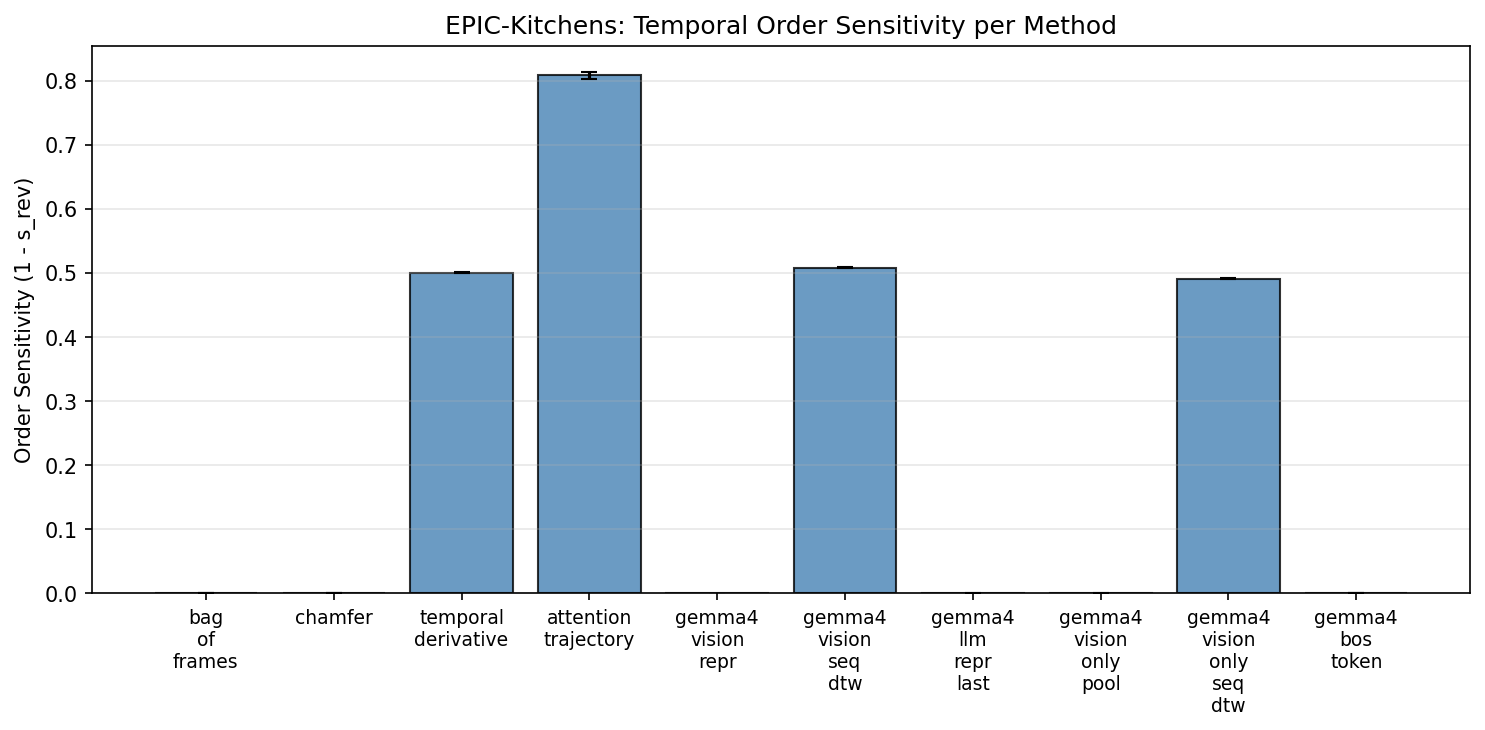
\includegraphics[width=0.95\textwidth]{../figures/epic_temporal_order_sensitivity.png}
    \caption{Comparator-specific $s_\text{rev}$ on EPIC-Kitchens. Cosine/Chamfer and DTW probes are separated because their numerical scales are not commensurate.}
    \label{fig:epic_sensitivity}
\end{figure}

\section{Cross-Method Summary Tables}
\label{sec:cross_method_tables}

This appendix consolidates per-method, per-benchmark AP and $s_\text{rev}$ values referenced throughout the main text. Table~\ref{tab:summary_encoders} reports dedicated encoders (DINOv3 and V-JEPA~2 variants, plus the temporal-training controls ViCLIP, X-CLIP, TARA, PL-Stitch, and an optical-flow baseline) on the four AP-scored benchmarks (VCDB, HDD, nuScenes, SSv2) and on EPIC reversal sensitivity. Table~\ref{tab:summary_vlm} reports the VLM probes grouped by pipeline stage (vision tower, pooled and per-frame sequence; pooled LLM hidden state) across the same benchmarks. The two tables are the source for the cross-regime claim of Section~\ref{sec:discussion}: no single method occupies the high-AP region for both copy detection and motion retrieval. Bootstrap CIs are in Appendix~\ref{sec:bootstrap_cis}; scene-matching extensions to Nymeria and MUVR are in Appendix~\ref{sec:scene_matching}.

\begin{table}[h]
\centering
\caption{Dedicated encoders across all tasks (VCDB: 5{,}585 pairs; HDD: 1{,}687 maneuvers; nuScenes: 950 pairs; SSv2: 400 chiral-pair clips; EPIC: 500 sequences). Nymeria and MUVR scene-matching results replicate the VCDB finding and are in Appendix~\ref{sec:scene_matching}. 95\% bootstrap CIs in Appendix~\ref{sec:bootstrap_cis}.}
\label{tab:summary_encoders}
\resizebox{\textwidth}{!}{%
\begin{tabular}{lccccc}
\toprule
\textbf{Method} & \textbf{VCDB (AP$\uparrow$)} & \textbf{HDD (AP$\uparrow$)} & \textbf{nuScenes (AP$\uparrow$)} & \textbf{SSv2 (AP$\uparrow$)} & \textbf{EPIC $s_\text{rev}$} \\
\midrule
DINOv3 BoF & 0.979 & 0.530 & 0.613 & 0.500 & 1.000 \\
DINOv3 Chamfer & \textbf{0.989} & 0.559 & 0.612 & 0.500 & 0.9999 \\
DINOv3 Temporal Deriv. & 0.775 & 0.498 & 0.623 & 0.503 & 0.500 \\
DINOv3 Attn.\ Trajectory & 0.700 & 0.507 & 0.584 & \textbf{0.720} & \textbf{0.192} \\
V-JEPA 2 BoT & 0.838 & 0.825 & 0.791 & 0.555 & 0.984 \\
V-JEPA 2 Encoder-Seq DTW & --- & 0.942 & \textbf{0.867} & --- & --- \\
V-JEPA 2 Temporal Res. & 0.698 & \textbf{0.956} & 0.815 & 0.556 & 0.0033 \\
ViCLIP (InternVid-10M) & 0.907 & 0.542 & 0.618 & --- & 0.996 \\
X-CLIP (16-frame) & 0.960 & --- & --- & --- & 0.980 \\
TARA (chiral, cosine) & --- & 0.547 & --- & --- & 0.955 \\
PL-Stitch BoF & --- & 0.478 & --- & --- & 1.000 \\
PL-Stitch DTW (raw emb.) & --- & 0.540 & --- & --- & 0.006 \\
Optical Flow (RAFT) DTW & --- & 0.478 & --- & --- & --- \\
\bottomrule
\end{tabular}
}
\begin{flushleft}
\small --- = not evaluated. VCDB AP depends on negative seed ($\pm$0.06; Appendix~\ref{sec:neg_sampling}). $s_\text{rev}$ values from cosine and DTW are not cross-comparable; V-JEPA~2 BoT uses cosine and its residual uses sequence DTW.
\end{flushleft}
\end{table}

\begin{table}[h]
\centering
\caption{VLM embedding probes across all tasks, grouped by pipeline stage. We report generative forward/reverse classification separately in Section~\ref{sec:vlm_generative} (Table~\ref{tab:vlm_generative}).}
\label{tab:summary_vlm}
\resizebox{\textwidth}{!}{%
\begin{tabular}{lcccc}
\toprule
\textbf{Method} & \textbf{VCDB (AP$\uparrow$)} & \textbf{HDD (AP$\uparrow$)} & \textbf{nuScenes (AP$\uparrow$)} & \textbf{EPIC $s_\text{rev}$} \\
\midrule
\multicolumn{5}{l}{\emph{Vision tower, pooled}} \\
Gemma-4 (SigLIP) & 0.926 & 0.521 & 0.662 & 1.000$^\dagger$ \\
LLaVA (CLIP) & 0.915 & 0.514 & 0.624 & 1.000$^\dagger$ \\
Qwen3-VL (SigLIP) & 0.491 & 0.421 & 0.464 & 0.998$^\dagger$ \\
\midrule
\multicolumn{5}{l}{\emph{Vision tower, per-frame sequence (DTW)}} \\
Gemma-4 (SigLIP) & 0.632 & 0.553 & 0.469 & 0.492 \\
LLaVA (CLIP) & 0.637 & 0.545 & 0.470 & 0.495 \\
Qwen3-VL (SigLIP) & 0.610 & 0.468 & 0.517 & 0.542 \\
\midrule
\multicolumn{5}{l}{\emph{LLM backbone, pooled hidden state}} \\
Gemma-4 & 0.838 & 0.472 & 0.569 & $\geq$0.998 \\
LLaVA & 0.907 & 0.512 & 0.652 & $\geq$0.998 \\
Qwen3-VL & 0.916 & 0.518 & 0.630 & $\geq$0.998 \\
\bottomrule
\end{tabular}
}
\begin{flushleft}
\small $^\dagger$Observed pooled cosine value, clamped to 1.000 where f32 precision exceeded one. Pooled and sequence rows use different comparators and numerical scales.
\end{flushleft}
\end{table}

\section{Full Scene Matching Results}
\label{sec:scene_matching}

We evaluated models across three scene-matching datasets: VCDB~\cite{vcdb} (copy detection), Nymeria~\cite{nymeria} (egocentric activity discrimination), and MUVR~\cite{muvr} (untrimmed multi-modal news/dance retrieval).

\begin{table}[h]
\centering
\caption{Retrieval AP driven by scene appearance / visual noise. VCDB: 528 videos, 5{,}585 positive pairs; Nymeria: 100 egocentric sessions, 8{,}780 segments; MUVR News: 9{,}958 videos, 74 topics.}
\label{tab:scene_matching}
\begin{tabular}{lccc}
\toprule
\textbf{Method} & \textbf{VCDB} & \textbf{Nymeria} & \textbf{MUVR (News)} \\
\midrule
\textbf{BoF (DINOv3)} & 0.979 & \textbf{0.485} & 0.731 \\
\textbf{Chamfer matching (DINOv3)} & \textbf{0.989} & 0.482 & \textbf{0.746} \\
Temporal Residual (V-JEPA 2) & 0.698 & 0.279 & 0.505 \\
Attention Trajectory (DINOv3) & 0.700 & 0.217 & 0.466 \\
\bottomrule
\end{tabular}
\end{table}

BoF and Chamfer have the largest point estimates in these three evaluations. On Nymeria they reach AP\,$\approx$\,0.48, and on MUVR News Chamfer reaches 0.746. Visual background is a plausible useful signal, but these aggregate pair results do not establish why the trajectory methods have lower AP.

\section{Preliminary: Qwen3-VL on VCDB}
\label{sec:qwen_vcdb}

We first tested whether VLMs can detect temporal reversal. Using Qwen3-VL~\cite{qwen3vl}, we presented forward and reversed versions of 49 VCDB videos and asked for temporal direction classification (3 trials each).

\begin{table}[h]
\centering
\caption{Qwen3-VL reversal detection on VCDB. Chance = 50\%.}
\label{tab:qwen_vcdb}
\begin{tabular}{llccc}
\toprule
\textbf{Model} & \textbf{Dataset (N)} & \textbf{Fwd Acc.} & \textbf{Rev Acc.} & \textbf{Overall} \\
\midrule
Qwen3-VL-4B-Instruct & Single clip (1) & 100\% & 0\% & 50.0\% \\
Qwen3-VL-30B-A3B & VCDB subset (49) & 83.0\% & 28.6\% & 55.8\% \\
\bottomrule
\end{tabular}
\end{table}

The 30B model achieves 55.8\%, near chance. The slight improvement is driven by a content-dependent FORWARD bias (83\% forward, 28.6\% reverse), not temporal understanding. This motivated the systematic multi-VLM evaluation on EPIC-Kitchens (Section~\ref{sec:vlm_generative}).

\section{VLM Temporal Integrity Probe}
\label{sec:integrity_probe}

Separately from forward/reverse classification, we asked VLMs to judge whether a video's temporal structure is ``INTACT'' or ``TAMPERED,'' on forward, reversed, and chunk-scrambled ($K\!=\!4, 16$) versions of EPIC-Kitchens sequences.

\begin{table}[h]
\centering
\caption{Temporal integrity probe on EPIC-Kitchens (500 sequences): fraction judged TAMPERED. LLaVA excluded from aggregate due to constant-output degeneracy.}
\label{tab:integrity_probe}
\begin{tabular}{lcccc}
\toprule
\textbf{Model} & \textbf{Forward} & \textbf{Reversed} & \textbf{Scramble $K\!=\!4$} & \textbf{Scramble $K\!=\!16$} \\
\midrule
Qwen3-VL-8B & 0.112 & 0.870 & 0.668 & 0.660 \\
Gemma-4-31B & 0.150 & 0.840 & 0.202 & 0.220 \\
LLaVA-Video-7B$^\dagger$ & 1.000 & 1.000 & 1.000 & 1.000 \\
\bottomrule
\end{tabular}
\begin{flushleft}
\small $^\dagger$LLaVA produces constant ``TAMPERED'' regardless of input (text-only baseline confirms). Excluded from integrity analysis.
\end{flushleft}
\end{table}

Qwen and Gemma identify forward videos as INTACT ($\sim$85--89\%) and flag reversed videos as TAMPERED (Qwen~87\%, Gemma~84\%). Treating forward as the negative class and reversed as the positive class gives balanced accuracy 0.879 for Qwen and 0.845 for Gemma. This directly contradicts a blanket claim that their outputs carry no temporal information: success depends strongly on the question and label framing. Scramble detection diverges, suggesting different heuristics. Cross-transform consistency is very low (3.8--8.2\%).

\section{VLM Prompt Sensitivity and Text-Only Baselines}
\label{sec:prompt_details}

Answers on direct forward/reverse classification are highly sensitive to prompt phrasing. Gemma-4 exhibits opposite biases across prompts: prompt~0 yields 87\% reverse bias; prompt~2 yields 73\% forward bias. LLaVA-Video answers ``FORWARD'' for prompts~0--1 ($>$98\%) but ``REVERSE'' for prompt~2 (83\%). Text-only baselines reproduce several of these priors; Qwen3 shows no text-only bias under the tested baseline but remains near chance with the direct video prompt.

LLaVA-Video produces constant ``TAMPERED'' regardless of input (text-only baseline confirms prior bias). We exclude it from aggregate integrity statistics in Appendix~\ref{sec:integrity_probe}.

\section{HDD Leakage Analysis}
\label{sec:hdd_leakage}

Since V-JEPA~2 temporal residuals achieve AP\,=\,0.956 on Honda HDD, above encoder-sequence DTW (0.942) and BoT (0.825), we test several potential shortcut explanations.

\textbf{Feature inputs.} All six methods receive \emph{only} decoded video frames. GPS is used exclusively for DBSCAN clustering; timestamps select the frame window ($\pm$3\,s) and are discarded before extraction.

\textbf{Segment duration.} Maneuver segments span 7.0--46.0\,s (mean 10.1\,s). Left and right turns have similar duration distributions (left: $10.3 \pm 3.8$\,s; right: $9.9 \pm 3.6$\,s), making duration an unlikely direct shortcut. V-JEPA~2 pads all segments to 64 frames, removing tensor length as an explicit signal, although duration still affects sampling density.

\textbf{Cluster composition.} Only ``mixed'' clusters containing both turn directions are used. Within each, all $\binom{n}{2}$ pairs are evaluated, ensuring models must distinguish maneuver type at the same location.

\textbf{Cross-session control.} To test session adjacency as one potential confound, we re-evaluate excluding same-session pairs (91.4\% of pairs are already cross-session). AP changes little: V-JEPA~2 temporal residual 0.957 (cross-session) vs.\ 0.956 (all pairs); BoF 0.536 vs.\ 0.530. This makes that specific explanation unlikely but does not rule out other correlations.

\textbf{Context-sensitivity control.} In the context sweep (Section~\ref{sec:context_sweep}), temporal-residual AP generally declines as padding widens, from 0.962 at $c\!=\!1$\,s to 0.838 at $c\!=\!8$\,s; BoT declines more sharply. Because padding changes visual context and sampling density together, this control does not identify a mechanism.

\textbf{Motion proxy check.} We compute mean pixel difference between consecutive frames for each segment and correlate pairwise proxy similarity with V-JEPA~2 residual similarity across all 97{,}731 pairs. Spearman $r = 0.051$; the motion proxy itself achieves AP\,=\,0.474. This argues against this particular motion-magnitude proxy as the explanation, but it does not identify what the residual encodes.

\section{VCDB Negative-Sampling Sensitivity}
\label{sec:neg_sampling}

Our primary VCDB evaluation uses 1:1 positive-to-negative sampling (5{,}585 pairs each). The full dataset contains $\binom{528}{2} \approx 139$K possible pairs. We re-evaluate at three ratios to verify robustness (Table~\ref{tab:neg_sensitivity}).

\begin{table}[h]
\centering
\caption{VCDB AP across negative-sampling ratios. \emph{Rank order and relative gaps are stable across all settings.} All-pairs uses the full $\binom{528}{2}$ set (requiring ${\sim}140$K DTW comparisons).}
\label{tab:neg_sensitivity}
\begin{tabular}{lccc}
\toprule
\textbf{Method} & \textbf{1:1} & \textbf{1:5} & \textbf{All pairs} \\
\midrule
DINOv3 Chamfer           & 0.989 & 0.949 & 0.845 \\
DINOv3 BoF               & 0.979 & 0.929 & 0.829 \\
DINOv3 Temporal Deriv.   & 0.775 & 0.424 & 0.228 \\
DINOv3 Attn.\ Trajectory & 0.700 & 0.408 & 0.225 \\
\bottomrule
\end{tabular}
\begin{flushleft}
\small Rank order (Chamfer $>$ BoF $>$ Temporal Deriv.\ $>$ Attn.\ Trajectory) is preserved across all ratios. AP decreases with more negatives as expected; AUC remains stable (e.g.\ Chamfer AUC: 0.990, 0.989, 0.989).
\end{flushleft}
\end{table}

\section{Bootstrap Confidence Intervals}
\label{sec:bootstrap_cis}

Table~\ref{tab:bootstrap} reports percentile intervals from resampling individual pairs (2{,}000 resamples, seed\,=\,42). Because pairs share clips and, for driving datasets, intersection clusters, these intervals do not have nominal 95\% coverage for independent experimental units and are retained only as descriptive resampling summaries. Degenerate samples fall back to the point estimate.

\begin{table}[h]
\centering
\caption{Descriptive pair-resampling percentile intervals for AP. ``Width'' is interval high minus low; narrow values can reflect dependence among pairs rather than low scientific uncertainty.}
\label{tab:bootstrap}
\begin{tabular}{llccc}
\toprule
\textbf{Benchmark} & \textbf{Method} & \textbf{AP} & \textbf{95\% CI} & \textbf{Width} \\
\midrule
\multirow{4}{*}{VCDB}
 & DINOv3 Chamfer           & 0.989 & [0.987, 0.991] & 0.004 \\
 & DINOv3 BoF               & 0.979 & [0.976, 0.981] & 0.005 \\
 & DINOv3 Temporal Deriv.   & 0.775 & [0.765, 0.784] & 0.019 \\
 & DINOv3 Attn.\ Trajectory & 0.700 & [0.689, 0.711] & 0.022 \\
 & V-JEPA 2 BoT             & 0.838 & [0.829, 0.846] & 0.017 \\
 & V-JEPA 2 Temporal Res.   & 0.698 & [0.687, 0.709] & 0.022 \\
\midrule
\multirow{6}{*}{HDD}
 & V-JEPA 2 Temporal Res.   & 0.956 & [0.955, 0.958] & 0.003 \\
 & V-JEPA 2 BoT             & 0.825 & [0.821, 0.828] & 0.007 \\
 & DINOv3 Chamfer           & 0.559 & [0.555, 0.564] & 0.009 \\
 & DINOv3 BoF               & 0.529 & [0.525, 0.534] & 0.009 \\
 & DINOv3 Attn.\ Trajectory & 0.507 & [0.502, 0.512] & 0.010 \\
 & DINOv3 Temporal Deriv.   & 0.498 & [0.494, 0.503] & 0.009 \\
\midrule
\multirow{7}{*}{nuScenes}
 & V-JEPA 2 Encoder-Seq DTW & 0.867 & [0.842, 0.890] & 0.048 \\
 & V-JEPA 2 Temporal Res.   & 0.815 & [0.785, 0.844] & 0.059 \\
 & V-JEPA 2 BoT             & 0.791 & [0.761, 0.820] & 0.059 \\
 & DINOv3 Temporal Deriv.   & 0.623 & [0.580, 0.665] & 0.085 \\
 & DINOv3 BoF               & 0.613 & [0.570, 0.658] & 0.088 \\
 & DINOv3 Chamfer           & 0.612 & [0.570, 0.659] & 0.089 \\
 & DINOv3 Attn.\ Trajectory & 0.584 & [0.540, 0.634] & 0.094 \\
\midrule
\multirow{6}{*}{Nymeria}
 & DINOv3 BoF               & 0.485 & [0.482, 0.489] & 0.007 \\
 & DINOv3 Chamfer           & 0.482 & [0.478, 0.485] & 0.007 \\
 & DINOv3 Temporal Deriv.   & 0.274 & [0.271, 0.277] & 0.006 \\
 & DINOv3 Attn.\ Trajectory & 0.217 & [0.215, 0.219] & 0.004 \\
 & V-JEPA 2 BoT             & 0.420 & [0.417, 0.424] & 0.007 \\
 & V-JEPA 2 Temporal Res.   & 0.278 & [0.276, 0.281] & 0.005 \\
\midrule
\multirow{6}{*}{MUVR News}
 & DINOv3 BoF               & 0.731 & [0.724, 0.740] & 0.016 \\
 & DINOv3 Chamfer           & 0.745 & [0.738, 0.754] & 0.016 \\
 & DINOv3 Temporal Deriv.   & 0.476 & [0.468, 0.485] & 0.017 \\
 & DINOv3 Attn.\ Trajectory & 0.466 & [0.458, 0.475] & 0.017 \\
 & V-JEPA 2 BoT             & 0.597 & [0.587, 0.605] & 0.018 \\
 & V-JEPA 2 Temporal Res.   & 0.505 & [0.496, 0.514] & 0.018 \\
\bottomrule
\end{tabular}
\begin{flushleft}
\small Pair-level intervals are especially narrow on HDD and Nymeria because many pairs reuse the same clips. On HDD, resampling intersection clusters instead widens the V-JEPA~2 temporal-residual interval from [0.955,\,0.958] to [0.890,\,0.978]. Marginal intervals do not test method differences; paired intersection-cluster contrasts for HDD and nuScenes are in Table~\ref{tab:paired_bootstrap}. Analogous independent-unit definitions are needed for VCDB, Nymeria, MUVR, and SSv2 before inferential claims.
\end{flushleft}
\end{table}

\begin{table}[h]
\centering
\caption{Paired intersection-cluster bootstrap differences in pooled pair AP (2{,}000 resamples). Intervals that include zero are not evidence of a directional difference.}
\label{tab:paired_bootstrap}
\begin{tabular}{llcc}
\toprule
\textbf{Dataset} & \textbf{Contrast (A $-$ B)} & \textbf{$\Delta$ AP} & \textbf{95\% interval} \\
\midrule
HDD & Encoder-Seq DTW $-$ BoT & +0.117 & [0.044, 0.127] \\
HDD & Temporal Residual $-$ Encoder-Seq DTW & +0.015 & [0.0004, 0.034] \\
HDD & Temporal Residual $-$ BoT & +0.132 & [0.048, 0.149] \\
\midrule
nuScenes & Encoder-Seq DTW $-$ BoT & +0.075 & [0.029, 0.128] \\
nuScenes & Encoder-Seq DTW $-$ Temporal Residual & +0.052 & [0.036, 0.064] \\
nuScenes & Temporal Residual $-$ BoT & +0.024 & [$-0.031$, 0.090] \\
\bottomrule
\end{tabular}
\end{table}

\section{DTW Similarity-Transform $\alpha$-Invariance}
\label{sec:alpha_sweep}

DTW similarities are computed as $s = \exp(-\alpha d)$ where $d$ is the accumulated cost normalized by $T_1+T_2$. For fixed positive $\alpha$, this is a strictly decreasing transformation of distance, so it cannot change a ranking-based metric such as AP apart from numerical ties. It \emph{does} change the numerical $s_\text{rev}$ scale, which is another reason not to compare those values across probe definitions. No empirical sweep with mismatched preprocessing is needed to establish this algebraic property.

\section{HDD Qualitative Analysis}
\label{sec:hdd_qualitative}

Complementing the quantitative results, we present qualitative evidence that V-JEPA~2 temporal residuals capture genuine motion dynamics rather than a visual shortcut.

\textbf{Nearest-neighbor examples.} For three representative intersection clusters, the top-3 neighbors by temporal residual similarity retrieve the same maneuver type despite identical backgrounds; errors occur when both turns share similar speeds through the same intersection phase.

\textbf{Background similarity statistics.} Within each GPS cluster, all segments share the same intersection. BoF cosine similarity for all $\binom{n}{2}$ pairs per cluster: mean $0.63 \pm 0.18$ (same-direction: $0.63 \pm 0.18$; cross-direction: $0.60 \pm 0.16$; gap = $0.029$), confirming appearance is non-discriminative. V-JEPA~2 temporal residual similarity aligns with maneuver labels (same: $0.008 \pm 0.006$; cross: $0.003 \pm 0.001$). Figure~\ref{fig:hdd_qualitative} shows the score distributions.

\begin{figure}[h]
\centering
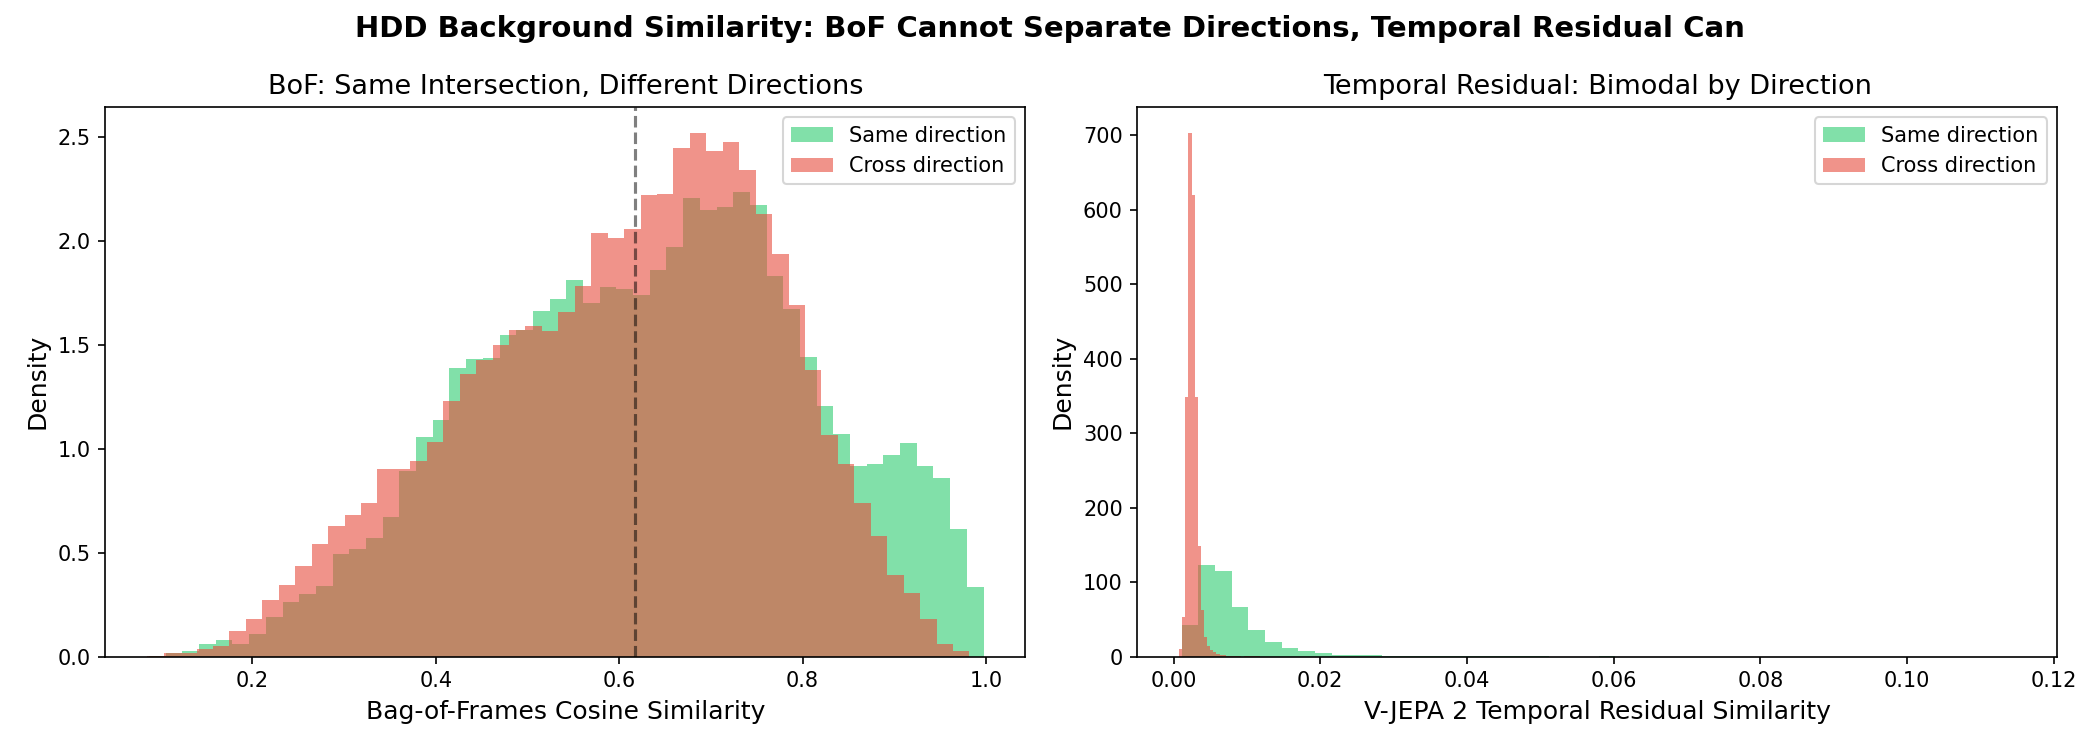
\includegraphics[width=\linewidth]{../figures/hdd_qualitative_distributions.png}
\caption{Pairwise similarity distributions on HDD intersection clusters. BoF similarities overlap heavily regardless of maneuver match, while V-JEPA~2 temporal residual scores separate same- vs.\ cross-direction pairs.}
\label{fig:hdd_qualitative}
\end{figure}

\section{BoT$\to$DTW Rerank: Corrected Directed Evaluation}
\label{sec:rerank_appendix}

The original experiment ranked unordered in-cluster pairs, admitted a pair when either endpoint survived, omitted out-of-cluster gallery negatives, and normalized AP by retrieved positives. Those choices could produce AP above recall and did not represent per-query retrieval. Table~\ref{tab:rerank_full} reports the replacement experiment.

\begin{table}[h]
\centering
\caption{Corrected directed HDD retrieval. Candidate recall is unchanged by reranking; AP@$k$ counts unreturned relevant items as misses.}
\label{tab:rerank_full}
\begin{tabular}{rccccc}
\toprule
$k$ & recall@$k$ & BoT AP@$k$ & DTW AP@$k$ & BoT MRR & DTW MRR \\
\midrule
10  & 0.165 & 0.127 & 0.109 & 0.761 & 0.700 \\
25  & 0.245 & 0.156 & 0.126 & 0.764 & 0.682 \\
50  & 0.331 & 0.176 & 0.136 & 0.765 & 0.665 \\
100 & 0.445 & 0.196 & 0.144 & 0.765 & 0.657 \\
250 & 0.651 & 0.223 & 0.156 & 0.766 & 0.645 \\
\bottomrule
\end{tabular}
\end{table}

For each query, the corrected gallery contains every other cached segment. Relevance requires both the same GPS cluster and the same maneuver label; all other segments are negatives. Metrics are macro-averaged over 1{,}673 eligible queries, with intersection-cluster bootstrap intervals. Full-gallery BoT mAP is 0.256 [0.218, 0.288] and full-gallery encoder-sequence-DTW mAP is 0.177 [0.135, 0.212]. At $k=100$, the BoT and reranked AP intervals are [0.175, 0.229] and [0.130, 0.160], respectively; reranking is worse throughout the sweep. The implementation is \texttt{experiments/eval\_hdd\_bof\_dtw\_rerank.py}.

\section{nuScenes Cross-Dataset Visualization}
\label{sec:nuscenes_figure}

Figure~\ref{fig:nuscenes_maneuver} visualizes the nuScenes maneuver-discrimination results reported in Section~\ref{sec:nuscenes}. Encoder-sequence DTW (AP\,=\,0.867) leads, followed by the temporal residual (AP\,=\,0.815) and BoT (AP\,=\,0.791), with DINOv3 methods below 0.625. Paired cluster contrasts support encoder-sequence DTW over both alternatives; the residual--BoT interval includes zero (Table~\ref{tab:paired_bootstrap}).

\begin{figure}[h]
    \centering
    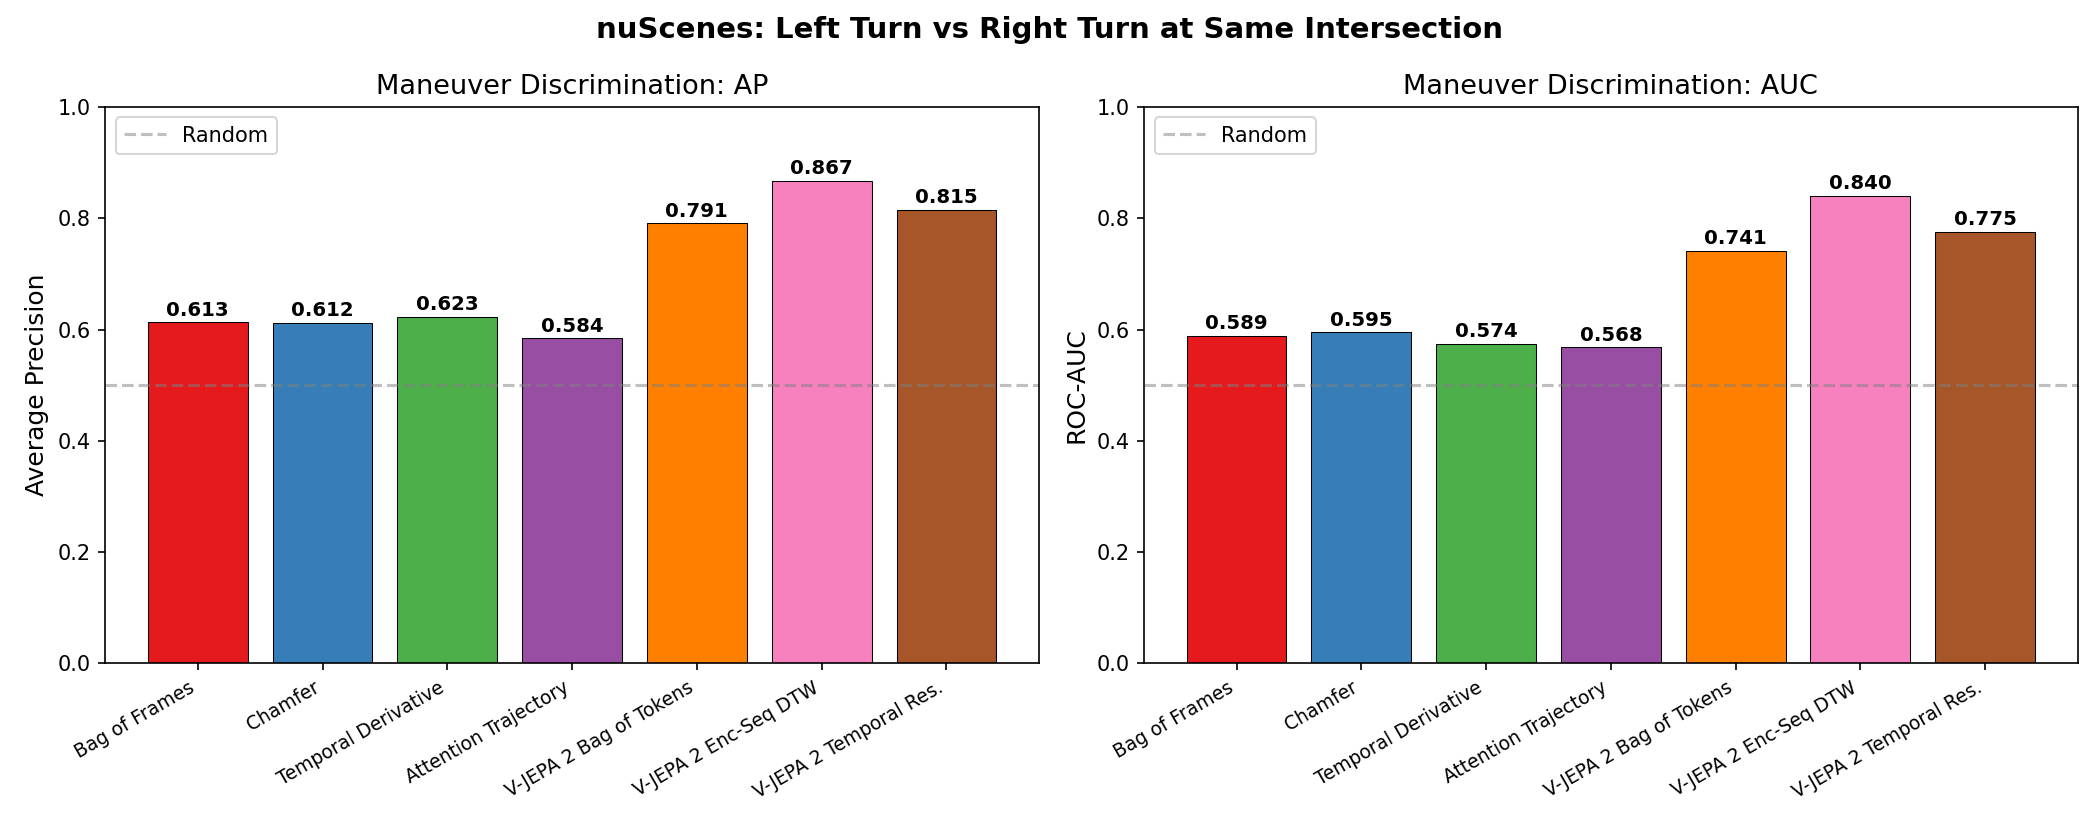
\includegraphics[width=0.9\textwidth]{../figures/nuscenes_maneuver_discrimination.png}
    \caption{nuScenes pair diagnostic (264 segments, 950 pairs, 50 intersection clusters). V-JEPA~2 encoder-sequence DTW has the largest AP (0.867); paired cluster contrasts are in Table~\ref{tab:paired_bootstrap}.}
    \label{fig:nuscenes_maneuver}
\end{figure}

\section{LLM Hidden-State Probe: Vision-Token-Only Analysis}
\label{sec:vision_token_probe}

A potential objection to our LLM hidden-state probe is that mean-pooling over \emph{all} tokens reintroduces symmetric aggregation. To address this, we extract LLM hidden states restricted to \emph{vision-token positions only}. Three variants:

\begin{enumerate}
    \item \textbf{Vision-only mean pool}: Mean-pool LLM hidden states at vision-token positions only. Compare via cosine similarity.
    \item \textbf{Vision-only per-frame sequence}: Group vision-token hidden states by their source frame, pool per frame to obtain a $(T, D)$ sequence. Compare via temporal derivative DTW.
    \item \textbf{BOS/first token}: Use the first token's hidden state (BOS or system token) as a summary representation. Compare via cosine similarity.
\end{enumerate}

\begin{table}[h]
\centering
\caption{$s_\text{rev}$ for vision-token-only LLM hidden-state probes (EPIC-Kitchens, 500 sequences). If vision-only pooling recovers temporal signal, we expect $s_\text{rev} \ll 1.0$; if order-invariance persists, the conclusion from Section~\ref{sec:vlm_embedding} is strengthened.}
\label{tab:vision_token_probe}
\begin{tabular}{lccc}
\toprule
\textbf{Model} & \textbf{Vision-only pool} & \textbf{Vision-only seq DTW} & \textbf{BOS token} \\
\midrule
Qwen3-VL-8B    & 0.998 [0.998, 0.998] & \textbf{0.542} [0.540, 0.544] & 0.996 \\
Gemma-4-31B    & 1.000 [1.000, 1.000]$^\dagger$ & \textbf{0.509} [0.509, 0.509] & 1.000 \\
LLaVA-Video-7B & 0.999 [0.998, 0.999] & \textbf{0.517} [0.516, 0.518] & 1.000$^\dagger$ \\
\bottomrule
\end{tabular}
\begin{flushleft}
\small Vision-only mean pooling yields cosine $s_\text{rev} \approx 1.0$ across all models, while the per-frame sequence probe yields lower values on a distinct DTW scale. This shows that sequence comparison detects forward/reverse changes that mean pooling suppresses; it does not establish a cross-comparator accuracy. BOS-token cosine is also near one under this probe. $^\dagger$Raw values $>$1.0 from f32 precision; clamped to 1.000.
\end{flushleft}
\end{table}

\section{Scramble Gradient Data}
\label{sec:scramble_data}

The original single-seed and raw-frame scripts formed $K-1$ short chunks plus one oversized tail when $T$ was not divisible by $K$ (for example, $T\!=\!30,K\!=\!16$ produced fifteen one-frame chunks and one fifteen-frame chunk). The corrected implementation uses near-equal partitions from \texttt{tensor\_split}/\texttt{array\_split}. Table~\ref{tab:scramble_data} reports means over 10 shuffle seeds.

\begin{table}[h]
\centering
\caption{Corrected AP across near-equal scramble partitions on VCDB (10 seeds). Across nontrivial $K$, the maximum standard deviation is 0.0101; invariant rows have zero variance.}
\label{tab:scramble_data}
\resizebox{\textwidth}{!}{%
\begin{tabular}{lcccccccc}
\toprule
\textbf{Method} & $K\!=\!1$ & $2$ & $3$ & $4$ & $6$ & $8$ & $12$ & $16$ \\
\midrule
BoF & 0.979 & 0.979 & 0.979 & 0.979 & 0.979 & 0.979 & 0.979 & 0.979 \\
Chamfer & 0.989 & 0.989 & 0.989 & 0.989 & 0.989 & 0.989 & 0.989 & 0.989 \\
Temporal Derivative & 0.775 & 0.730 & 0.733 & 0.730 & 0.726 & 0.725 & 0.725 & 0.726 \\
Attention Trajectory & 0.700 & 0.636 & 0.626 & 0.618 & 0.603 & 0.594 & 0.583 & 0.575 \\
V-JEPA~2 BoT & 0.837 & 0.837 & 0.837 & 0.837 & 0.837 & 0.837 & 0.837 & 0.837 \\
V-JEPA~2 Temporal Residual & 0.698 & 0.597 & 0.628 & 0.614 & 0.632 & 0.626 & 0.631 & 0.633 \\
\bottomrule
\end{tabular}
}
\end{table}

The extracted-embedding gradient tests the comparator's response while keeping token values fixed. The raw-frame variant re-encodes each shuffled video and therefore measures the combined encoder and comparator response. Under raw-frame scrambling, V-JEPA~2 BoT remains approximately flat (0.839 at $K\!=\!1$, 0.840 at $K\!=\!16$), while residual AP falls from 0.705 to 0.651. This supports combined encoder--comparator sensitivity but does not make the extracted-embedding residual curve monotonic.

\section{Linear Probe on LLM Hidden States}
\label{sec:linear_probe}

The $s_\text{rev}$ analysis (Section~\ref{sec:vlm_embedding}) shows that mean-pooled LLM hidden states are order-invariant. A natural follow-up: is temporal signal present in the per-position hidden states but lost to symmetric aggregation? If so, a learned classifier should recover it.

We extract last-layer hidden states from all three VLMs for 200 EPIC-Kitchens sequences (forward and reverse), yielding 400 samples per model. We train $\ell_2$-regularized logistic regression (5-fold GroupKFold CV, fwd/rev pairs kept together, $C \in \{0.01, 0.1, 1, 10, 100\}$) on seven readout strategies:

\begin{itemize}
    \item \textbf{mean}: mean over all positions (replicates $s_\text{rev}$ finding)
    \item \textbf{max}: element-wise max over all positions
    \item \textbf{first} / \textbf{last}: single position (BOS or final token)
    \item \textbf{concat\_first\_last}: concatenation of first and last positions
    \item \textbf{vision\_mean}: mean restricted to vision-token positions
    \item \textbf{vision\_concat\_fl}: first and last vision-token positions
\end{itemize}

\begin{table}[h]
\centering
\caption{Exploratory probe accuracy (GroupKFold CV, fwd/rev pairs kept together) for forward vs.\ reverse classification from LLM hidden states. Linear reports the best observed $C \in \{0.01, 0.1, 1, 10, 100\}$ on the same CV folds; MLP is a 2-layer network. Chance = 0.500. No nested-CV or held-out selection correction is applied.}
\label{tab:linear_probe}
\resizebox{\textwidth}{!}{%
\begin{tabular}{lcccccc}
\toprule
& \multicolumn{2}{c}{\textbf{Gemma-4 31B}} & \multicolumn{2}{c}{\textbf{LLaVA-Video 7B}} & \multicolumn{2}{c}{\textbf{Qwen3-VL 8B}} \\
\cmidrule(lr){2-3} \cmidrule(lr){4-5} \cmidrule(lr){6-7}
\textbf{Pooling} & \textbf{Linear} & \textbf{MLP} & \textbf{Linear} & \textbf{MLP} & \textbf{Linear} & \textbf{MLP} \\
\midrule
mean                & 0.512 & 0.552 & 0.500 & 0.505 & 0.537 & 0.510 \\
max                 & 0.532 & 0.458 & 0.470 & 0.490 & 0.528 & 0.502 \\
first               & 0.500 & 0.500 & 0.500 & 0.500 & 0.500 & 0.500 \\
last                & 0.510 & 0.507 & 0.515 & 0.495 & 0.550 & 0.512 \\
concat\_first\_last & 0.515 & 0.490 & 0.505 & 0.478 & 0.555 & 0.520 \\
vision\_mean        & 0.520 & 0.550 & 0.502 & 0.512 & 0.537 & 0.505 \\
vision\_concat\_fl  & 0.528 & 0.500 & 0.495 & 0.467 & 0.515 & 0.535 \\
\bottomrule
\end{tabular}
}
\end{table}

The observed accuracies range from 0.458 to 0.560. Given the 126 explored configurations, reuse of CV folds for hyperparameter selection, and lack of a permutation test or held-out confirmation set, these results provide no reliable evidence that a fixed-dimensional readout decodes direction; they also cannot establish absence. The ``first'' token gives exactly 0.500 when its input is identical across conditions, providing a basic pipeline check.

Per-position LLM hidden states do change detectably under sequence DTW ($s_\text{rev} \approx 0.51$--$0.54$ on that probe's scale; Table~\ref{tab:vision_token_probe}). The current experiment therefore supports a readout-dependence claim, not the stronger assertion that no fixed-dimensional reduction can retain order.

\section{Computational Costs}
\label{sec:computational_costs}

Table~\ref{tab:costs} summarizes approximate per-video extraction and per-pair comparison costs on a single H200 GPU. Feature extraction is a one-time index-build cost, while comparison cost governs query latency. End-to-end latency and quality depend on the corrected directed retrieval evaluation and are not inferred from pair timing alone.

\begin{table}[h]
\centering
\caption{Per-video feature extraction and per-pair comparison costs on a single H200 GPU. $T$ = number of frames per clip.}
\label{tab:costs}
\begin{tabular}{lcc}
\toprule
\textbf{Method} & \textbf{Extraction (ms/video)} & \textbf{Comparison (ms/pair)} \\
\midrule
DINOv3 BoF ($T\!=\!30$) & ${\sim}120$ & $<$0.01 (cosine) \\
DINOv3 Chamfer ($T\!=\!30$) & ${\sim}120$ & ${\sim}0.3$ (frame matrix) \\
DINOv3 Attn.\ Trajectory ($T\!=\!30$) & ${\sim}150$ & ${\sim}1$ (DTW) \\
DINOv3 Temporal Deriv.\ ($T\!=\!30$) & ${\sim}120$ & ${\sim}1$ (DTW) \\
V-JEPA 2 BoT ($T\!=\!64$) & ${\sim}280$ & $<$0.01 (cosine) \\
V-JEPA 2 Temporal Res.\ ($T\!=\!64$) & ${\sim}560$ & ${\sim}1$ (DTW) \\
VLM vision pooled & ${\sim}800$--$2{,}500$ & $<$0.01 (cosine) \\
VLM LLM hidden state & ${\sim}1{,}500$--$5{,}000$ & $<$0.01 (cosine) \\
\bottomrule
\end{tabular}
\begin{flushleft}
\small V-JEPA~2 temporal residual requires both encoder and predictor forward passes, roughly doubling extraction cost vs.\ BoT. DTW comparison at $T \approx 30$ is ${\sim}1$\,ms, so reranking 100 candidates adds roughly 100\,ms of comparator time. This microbenchmark is not a production-readiness claim.
\end{flushleft}
\end{table}

\section{Failure-Mode Taxonomy}
\label{sec:failure_taxonomy}

The diagnostic suite's value is not individual numbers but a structured classification of \emph{why} video retrieval systems fail temporally. We categorize every failure surfaced in Sections~3 and~4 into six failure classes; four classes (A, D, E, F) admit a secondary variant (A$'$, D$'$, E$'$, F$'$) attested by the data, yielding ten rows in Table~\ref{tab:failure_taxonomy}.

\begin{table}[h]
\centering
\small
\caption{Failure-mode taxonomy. Each row names an observed diagnostic pattern and a possible locus from the seven-benchmark evaluation. Multiple patterns can occur in one system.}
\label{tab:failure_taxonomy}
\begin{tabular}{p{0.7cm}p{2.0cm}p{3.8cm}p{5.4cm}}
\toprule
\textbf{Class} & \textbf{Possible locus} & \textbf{Diagnostic symptom} & \textbf{Canonical instance} \\
\midrule
\textbf{(A)} & Architectural & Symmetric aggregation of fixed elements gives exact permutation invariance & DINOv3 BoF and Chamfer \\
\textbf{(A$'$)} & Contextual readout & Pooled cosine is near one although token values may depend on order & Pooled VLM vision/LLM probes \\
\textbf{(B)} & Feature--task mismatch & Comparator changes do not yield strong task discrimination & DINOv3 HDD AP\,$\leq$\,0.559 \\
\textbf{(C)} & Comparator--task mismatch & Low self-reversal similarity does not imply high task AP & PL-Stitch HDD DTW 0.540 despite $s_\text{rev}\!=\!0.006$ \\
\textbf{(D)} & Context / density & Context sweep changes two factors jointly & V-JEPA 2 gap: $+0.038$ at $c\!=\!1$\,s $\to +0.224$ at $c\!=\!8$\,s \\
\textbf{(D$'$)} & Sampling density & Fixed low frame cap confounds cross-encoder comparison & ViCLIP 8-frame input, ${\sim}0.20$ AP drop at equivalent density \\
\textbf{(E)} & Evaluation protocol & Pair-level CIs underestimate width under cluster-structured pairs & HDD pair-level $[0.955, 0.958]$ vs.\ cluster-level $[0.890, 0.978]$ \\
\textbf{(E$'$)} & Evaluation protocol & Seed-dependent absolute AP masks true rank order & VCDB AP drifts ${\pm}0.06$ across negative seeds (Appendix~\ref{sec:neg_sampling}) \\
\textbf{(F)} & Behavioral / output & Generative output obscures internal temporal signal & Gemma-4: 87\% reverse bias on prompt 0 $\to$ 73\% forward bias on prompt 2 (Appendix~\ref{sec:prompt_details}) \\
\textbf{(F$'$)} & Behavioral / output & Pooled-readout null $\ne$ absence of signal ($p\!\gg\!n$) & Exploratory fixed-vector probes are weak; sequence DTW detects changes \\
\bottomrule
\end{tabular}
\end{table}

Two design choices make this taxonomy actionable rather than descriptive. First, the classes are \emph{tool-indexed}: (A)/(A$'$) surface under the reversal test, (C) under the decomposition, (D) under the context sweep, (E) under cluster bootstrap, (F) under generative-vs-embedding probe disagreement. A practitioner running \textsc{TemporalDiag} on a new system can map diagnostic outputs onto failure classes without reading Section~3. Second, the classes are non-exclusive: BoF fails on (A) and (B); Qwen3-VL fails on (A$'$); pair-level CI claims fail on (E). This compositionality lets us distinguish systems that would look identical under a single-metric evaluation.

\section{Reproducibility Appendix}
\label{sec:reproducibility}

This appendix documents inputs, intended use, and known limitations of the \textsc{TemporalDiag} diagnostic suite to support reproduction of our experiments. It is not a datasheet for a released dataset (we release no new data) but a scope statement for a diagnostic toolkit applied to seven existing public benchmarks.

\textbf{Scope and intended use.} \textsc{TemporalDiag} accepts per-frame embeddings or sequence representations from any vision or VLM encoder, plus pairwise ground-truth labels, and emits (i)~a scramble-gradient profile (AP vs.\ $K\in\{1,\ldots,16\}$), (ii)~a reversal-sensitivity score $s_\text{rev}$ under a user-chosen similarity function, and (iii)~optional feature-vs-comparator decomposition outputs when per-frame and pooled variants of the same encoder are supplied. The toolkit is intended for diagnostic analysis of video retrieval systems whose primary metric is pairwise AP/AUC on same/different-category labels. It is \emph{not} intended to score or rank systems on a closed leaderboard.

\textbf{Inputs.} Embeddings are \texttt{\{video\_id: (T, D)\}} dictionaries in PyTorch \texttt{.pt} format; pair lists are CSVs with \texttt{(id\_a, id\_b, label)} tuples. Supported similarity functions are cosine, Chamfer (symmetric-max aggregation), and DTW with configurable $\alpha$ (Equation~\ref{eq:srev}). DTW uses unconstrained warping, L2 cost, accumulated-cost normalization by $T_1+T_2$, and GPU-vectorized anti-diagonal wavefront processing.

\textbf{Seeds, splits, and variance.} Unless specified, all randomness is controlled by seed~42. The corrected scramble uses 10 shuffle seeds per $K$; pair and grouped cluster bootstraps use 2{,}000 resamples, while EPIC reversal intervals use 1{,}000. Negative-sampling is seeded in VCDB; sensitivity across seeds yields $\pm0.06$ AP drift (Appendix~\ref{sec:neg_sampling}), with rank order preserved. No train/val/test split is needed because the suite evaluates frozen models zero-shot.

\textbf{Known limitations.} (1)~Pair-level bootstrap CIs underestimate uncertainty by 7--32$\times$ under GPS-clustered pair sets; we use paired intersection-cluster bootstrap on HDD and nuScenes (Appendix~\ref{sec:bootstrap_cis}), but analogous independent units remain undefined for several other datasets. (2)~Probe analyses run in a $p\gg n$ regime (400 samples, $D\approx4{,}000$), bounding recoverability rather than proving absence. (3)~Cross-family $s_\text{rev}$ comparisons (pooled cosine vs.\ sequence DTW) are not unit-commensurate. (4)~Qwen3-VL's 3D temporal--spatial merging prevents clean per-frame token grouping (Table~\ref{tab:vlm_embedding} footnote); approximate values are flagged.

\textbf{Reproduction recipe.} Experiment entry points and required caches are documented in \texttt{REPRODUCIBILITY.md}. Compact corrected summaries and their commit, job, dataset, and model provenance are tracked under \texttt{results/}; feature caches remain external because of their size and dataset licenses. The supplied SLURM jobs regenerate the balanced-chunk scramble, EPIC residual, grouped bootstrap contrasts, and directed HDD retrieval results.

\textbf{License.} Code is released under the MIT License. Dataset and model-weight licenses are summarized in Appendix~\ref{sec:licenses}; users must independently obtain each asset under its own license terms.

\section{Dataset and Model Licenses}
\label{sec:licenses}

All experiments use publicly available datasets and pretrained models. Table~\ref{tab:licenses} lists the governing license for each asset. Use is restricted to non-commercial research, consistent with the most restrictive license among the assets combined in any given experiment. No new datasets or model weights are released by this paper.

\begin{table}[h]
\centering
\small
\caption{Licenses for datasets and pretrained model weights used in this work. Verbatim license text is available from each asset's canonical distribution channel; see \texttt{REPRODUCIBILITY.md} for HuggingFace IDs and download URLs.}
\label{tab:licenses}
\begin{tabular}{lll}
\toprule
\textbf{Asset} & \textbf{License} & \textbf{Distribution} \\
\midrule
\multicolumn{3}{l}{\emph{Datasets}} \\
VCDB~\cite{vcdb}                      & Research-only; no warranty (Fudan Univ.)    & Project page \\
Honda HDD~\cite{honda_hdd}            & HRI-USA Data Use Agreement (non-commercial) & HRI-USA \\
nuScenes~\cite{nuscenes}              & CC BY-NC-SA 4.0                             & nuscenes.org \\
EPIC-Kitchens-100~\cite{epickitchens} & CC BY-NC 4.0                                & epic-kitchens.github.io \\
Nymeria~\cite{nymeria}                & CC BY-NC 4.0                                & facebookresearch GH \\
MUVR~\cite{muvr}                      & Research-only (authors' terms)              & Authors' release \\
\midrule
\multicolumn{3}{l}{\emph{Pretrained model weights}} \\
DINOv3~\cite{dinov3}                  & Meta FAIR non-commercial                    & HuggingFace \\
V-JEPA~2~\cite{vjepa2}                & CC BY-NC 4.0                                & HuggingFace \\
ViCLIP / InternVid~\cite{viclip}      & Apache 2.0 (code); CC BY-NC 4.0 (weights)   & OpenGVLab \\
X-CLIP~\cite{xclip}                   & MIT                                         & microsoft/VideoX \\
Qwen3-VL-8B~\cite{qwen3vl}            & Apache 2.0                                  & HuggingFace \\
Gemma~4~\cite{gemma4}                 & Gemma Terms of Use                          & HuggingFace \\
LLaVA-Video~\cite{llavavideo}         & Apache 2.0 (code); Llama-2 terms (weights)  & HuggingFace \\
RAFT (optical flow)                   & BSD-3-Clause                                & princeton-vl/RAFT \\
\bottomrule
\end{tabular}
\end{table}

Honda HDD access required a signed Data Use Agreement with HRI-USA; nuScenes required account registration at nuscenes.org; other datasets are downloadable under their respective non-commercial licenses. All assets were used for non-commercial research evaluation only.

\end{document}
